\documentclass[12pt,oneside]{article}

%%%%%%%%%%%%%%%%%%%%%%%%%%%%
%%   Zusaetzliche Pakete  %%
%%%%%%%%%%%%%%%%%%%%%%%%%%%%
\usepackage{acronym}
\usepackage{enumerate}
\usepackage{a4wide}
\usepackage{fancyhdr}
\usepackage[pdftex]{graphicx}
\usepackage{palatino}
%\usepackage{blindtext}
\usepackage{multirow}
%\usepackage[ruled,longend]{algorithm2e}
\usepackage{float}
\usepackage{amsmath}
\usepackage{amssymb}
\usepackage{listings}
\usepackage[numbib]{tocbibind}

%folgende Zeile auskommentieren für englische Arbeiten
\usepackage[ngerman]{babel}

\usepackage[bookmarks]{hyperref}
\usepackage[T1]{fontenc}
\usepackage[utf8]{inputenc}
\usepackage[a-1b]{pdfx}
\usepackage[justification=centering]{caption}
%\usepackage[style=unsrt,natbib=true,backend=biber]{biblatex}
\usepackage{csquotes}
\usepackage{url}
%\usepackage{subfigure}
% Layout corrections (Schusterjungen)
\clubpenalty = 10000 
% Layout corrections (Hurenkinder) 
\widowpenalty = 10000 
\displaywidowpenalty = 10000
\emergencystretch=1em

% Figures
\usepackage[hypcap=true,labelformat=simple]{subcaption}
\renewcommand{\thesubfigure}{(\alph{subfigure})}

% Tables
\usepackage{booktabs} 

% Newcommand TODO (red in text)
\newcommand{\todo}[1]{\textcolor{red}{TODO: #1}}

% Newcommand TODOM (red at border)
\newcommand{\todom}[1]{\marginpar{\parbox{1.5cm}{\textcolor{red}{TODO:\\ #1}}}}





%%%%%%%%%%%%%%%%%%%%%%%%%%%%%%
%% Definition der Kopfzeile %%
%%%%%%%%%%%%%%%%%%%%%%%%%%%%%%

\pagestyle{fancy}
\fancyhf{}
\cfoot{\thepage}
\setlength{\headheight}{16pt}

%%%%%%%%%%%%%%%%%%%%%%%%%%%%%%%%%%%%%%%%%%%%%%%%%%%%%
%%  Definition des Deckblattes und der Titelseite  %%
%%%%%%%%%%%%%%%%%%%%%%%%%%%%%%%%%%%%%%%%%%%%%%%%%%%%%

\newcommand{\HSFTitle}[8]{

  \thispagestyle{empty}
\begin{center}
    
\includegraphics[width=0.9\textwidth]{logo_new_2.png} \\
    \vspace*{\stretch{1}}
    \end{center}

  %\vspace*{\stretch{1}}
  {\parindent0cm
  \rule{\linewidth}{.7ex}}
  \begin{center}
    \vspace*{\stretch{1}}
    \sffamily\bfseries\Huge
    #1\\
    \vspace*{\stretch{1}}
    \sffamily\bfseries\large
    #3
    \vspace*{\stretch{1}}
  \end{center}
  \rule{\linewidth}{.7ex}

  \vspace*{\stretch{2}}
  \begin{center}
    \Large #2 am #5 der HS Fulda \\
    \vspace*{\stretch{1}}

    \large Matrikelnummer:  #4 \\[1mm]
    \large Erstbegutachtung:  #7 \\[1mm]
    \large Zweitbegutachtung:  #8 \\[1mm]

    \vspace*{\stretch{1}}
    \large Eingereicht am #6
  \end{center}
}


%%%%%%%%%%%%%%%%%%%%%%%%%%%%
%%  Beginn des Dokuments  %%
%%%%%%%%%%%%%%%%%%%%%%%%%%%%

\begin{document}

  \HSFTitle
      {Embedding-basierte Analyse von Kompetenzformulierungen -- Potenziale eines hybriden Ansatzes mit regelbasierter Textanalyse}        % Titel der Arbeit
      {Masterarbeit} % Typ der Arbeit
      {Felix Beinssen}          % Vor- und Nachname der Autor*in
      {1522578}
      {Fachbereich AI}  % Name des FBs
      {31.07.2026}        % Tag der Abgabe
      {Prof. Dr.-Ing. Johannes Konert}     % Name der Erstgutachter*in
      {Cathrin Möller}    % Name der Zweitgutachter*in

  \clearpage

\lhead{}
\pagenumbering{Roman}
    \setcounter{page}{1}

%%%%%%%%%%%%%%%%%%%%%%%%%%%%
%%  Kurzzusammenfassung   %%
%%%%%%%%%%%%%%%%%%%%%%%%%%%%
\clearpage
%
\markboth{Abstract}{Abstract}
\section*{Abstract}
Modulhandbücher deutschsprachiger Hochschulen enthalten Kompetenzformulierungen, die beschreiben, welche Fähigkeiten Studierende nach Abschluss eines Moduls erworben haben sollen.
Die Qualität dieser Formulierungen variiert erheblich: Nicht alle Sätze enthalten beobachtbare Handlungsverben, und die Zuordnung zu kognitiven Taxonomiestufen nach Anderson und Krathwohl ist häufig unklar.
Ein bestehender regelbasierter Prototyp unterstützt Lehrende bei der Analyse solcher Formulierungen durch exakten Abgleich mit einer statischen Verbliste, stößt jedoch an strukturelle Grenzen, wenn Verben nicht in der Liste enthalten sind.

Diese Arbeit untersucht, welche Potenziale ein Embedding-basierter Ansatz gegenüber regelbasierter Textanalyse für die Unterstützung Lehrender bietet.
Dazu werden drei Ansätze -- regelbasiert, Embedding-basiert (Sentence-BERT mit SVM-Klassifikation) und ein hybrider Cascading-Ansatz -- entworfen, in einem webbasierten Editor (Nuxt~4, FastAPI) implementiert und auf einem Gold-Standard-Datensatz von 5\,617~Sätzen aus Modulhandbüchern mehrerer deutscher Hochschulen evaluiert, wobei eine Institution den Schwerpunkt bildet.

Der Embedding-Ansatz erreicht $F_1 = 0{,}963$ bei der Satztyp-Klassifikation und $F_1 = 0{,}839$ bei der Taxonomie-Zuordnung -- deutlich über dem regelbasierten Ansatz ($F_1 = 0{,}819$ bzw.\ $0{,}581$) und mit vollständiger Abdeckung statt 48{,}2\,\%.
Der hybride Cascading-Ansatz ($F_1 = 0{,}929$ bzw.\ $0{,}713$) bleibt hinter dem reinen Embedding-Ansatz zurück, da Fehlerfortpflanzung im Cascading den theoretischen Transparenzvorteil überwiegt.
Die semantische Repräsentation ermöglicht darüber hinaus ein Empfehlungssystem (Precision@1 $= 0{,}510$) und eine Taxonomie-Abdeckungsanalyse auf Modulebene -- Funktionen, die mit dem regelbasierten Ansatz nicht realisierbar sind.
Die Konfidenzwerte der SVM-Klassifikation erweisen sich als brauchbarer Qualitätsindikator: Bei hoher Konfidenz ($\geq 0{,}8$) steigt der Typ-F1 auf $0{,}986$.
\clearpage
\tableofcontents
\clearpage

%\addcontentsline{toc}{section}{\listfigurename}
\listoffigures

%\addcontentsline{toc}{section}{\listtablename}
\listoftables
\clearpage


%%%%%%%%%%%%%%%%%%%%%%%%%%%%
%%  Einstellungen  %%
%%%%%%%%%%%%%%%%%%%%%%%%%%%%
\cleardoublepage
\pagenumbering{arabic}
    \setcounter{page}{1}
\lhead{\nouppercase{\leftmark}}

%%%%%%%%%%%%%%%%%%%%%%%%%%%%
%%  Hauptteil  %%
%%%%%%%%%%%%%%%%%%%%%%%%%%%%

\section{Einleitung}\label{sec:einleitung}
% =============================================================================
% Kapitel 1: Einleitung
% =============================================================================

Dieses Kapitel führt in den Gegenstand der Arbeit ein, motiviert die Forschungsfrage und gibt einen Überblick über den Aufbau der Thesis.

\subsection{Kontext}\label{sec:kontext}

Die Qualität der Hochschullehre hängt wesentlich davon ab, wie präzise Lehrende beschreiben, was Studierende am Ende eines Moduls wissen und können sollen.
Mit dem Bologna-Prozess vollzog sich in der europäischen Hochschullandschaft ein grundlegender Paradigmenwechsel: weg von einer Input-Orientierung, die beschreibt, \emph{was gelehrt wird}, hin zu einer Output-Orientierung, die formuliert, \emph{was Studierende nach Abschluss eines Lernprozesses in der Lage sind zu tun}~\cite{hrknexus2015lernergebnisse}.
Modulhandbücher, in denen die Qualifikationsziele jedes Studienmoduls festgehalten werden, sind das zentrale Instrument dieser Kompetenzorientierung.
Die Kultusministerkonferenz und die Hochschulrektorenkonferenz haben mit dem Qualifikationsrahmen für deutsche Hochschulabschlüsse~\cite{kmk2017qualifikationsrahmen} sowie dem Deutschen Qualifikationsrahmen~\cite{dqr2013handbuch} verbindliche Rahmenvorgaben geschaffen, die eine einheitliche Beschreibung von Lernergebnissen auf verschiedenen Niveaustufen verlangen.

Was eine gute Kompetenzformulierung ausmacht, ist in der Fachliteratur gut beschrieben.
Weinert definiert Kompetenzen als \glqq die bei Individuen verfügbaren oder durch sie erlernbaren kognitiven Fähigkeiten und Fertigkeiten, um bestimmte Probleme zu lösen, sowie die damit verbundenen motivationalen, volitionalen und sozialen Bereitschaften und Fähigkeiten\grqq~\cite{weinert2001leistungsmessung}.
Schaper et al.\ operationalisieren diesen Begriff für den akademischen Kontext und fordern, dass Kompetenzformulierungen konkretes, beobachtbares Handeln beschreiben~\cite{schaper2012fachgutachten}.
Der Praxisleitfaden der HRK konkretisiert dies weiter: Eine Kompetenzformulierung benennt die Studierenden als Subjekt, enthält genau ein beobachtbares Handlungsverb und spezifiziert den fachlichen Gegenstand der Handlung~\cite{hrknexus2015lernergebnisse}.

Für die systematische Einordnung dieser Handlungsverben hat sich die Taxonomie kognitiver Prozesse nach Anderson und Krathwohl~\cite{anderson2001taxonomy} als Standard etabliert.
Sie unterscheidet sechs hierarchische Stufen kognitiver Komplexität: \emph{Erinnern}, \emph{Verstehen}, \emph{Anwenden}, \emph{Analysieren}, \emph{Bewerten} und \emph{Erschaffen}.
Die Zuordnung von Kompetenzformulierungen zu diesen Stufen ermöglicht es, das Anforderungsniveau einzelner Module transparent zu machen und die Abdeckung verschiedener kognitiver Prozesse innerhalb eines Studiengangs zu überprüfen.
Krathwohl betont dabei die Zweidimensionalität der Taxonomie: Neben dem kognitiven Prozess (kodiert durch das Verb) bestimmt auch die Wissensdimension (kodiert durch den Inhalt) das Anspruchsniveau einer Formulierung~\cite{krathwohl2002revision}.

In der Praxis stehen Lehrende beim Verfassen von Modulhandbüchern jedoch vor einer anspruchsvollen Aufgabe.
Sie müssen nicht nur fachlich korrekte Inhalte formulieren, sondern diese auch in einer Form niederschreiben, die den Qualitätskriterien kompetenzorientierter Lernergebnisse genügt.
Schaper et al.\ stellen fest, dass Kompetenzformulierungen in Modulhandbüchern \glqq teilweise willkürlich und ohne klare Bezüge zu Zieltaxonomien oder Kompetenzanalysen\grqq\ vorgenommen werden~\cite{schaper2012fachgutachten}.
Softwaregestützte Werkzeuge, die Lehrende beim Formulieren unterstützen und automatisiertes Feedback zur Qualität ihrer Kompetenzformulierungen geben, können diese Situation verbessern.

%
\subsection{Problemstellung und Motivation}\label{sec:problemstellung}

Ein bestehender Prototyp von Loth und Konert~\cite{loth2022kompetenzeditor} adressiert dieses Problem durch regelbasierte Echtzeitanalyse in einem webbasierten Editor: Verben werden mittels spaCy tokenisiert, per exaktem Stringvergleich gegen eine statische Liste von rund 80~Handlungsverben abgeglichen und farblich hervorgehoben.
Bei nicht empfohlenen Verben wird eine generische Tabelle empfohlener Alternativen angezeigt.
Dieser Ansatz bietet Transparenz -- jede Zuordnung ist direkt auf ein Verb und eine Listenregel zurückführbar -- und funktioniert zuverlässig für die Verben, die in der Liste enthalten sind.

Drei strukturelle Probleme begrenzen jedoch die Analysequalität.
Erstens sind die Listen \emph{geschlossen}: Jedes Verb, das nicht in der Liste vorkommt, wird nicht analysiert, obwohl es durchaus eine valide Kompetenzformulierung sein kann.
Ungewöhnliche Synonyme, fachspezifische Verben oder Komposita bleiben unerkannt.
Die Autoren selbst identifizieren in ihrem Fazit die Notwendigkeit, Schlüsselwörter auch in abgewandelter Form zu analysieren und Texte mit Referenzformulierungen vergleichen zu können~\cite{loth2022kompetenzeditor}.
Zweitens liefert ein reiner Stringvergleich \emph{keine Kontextinformation}.
Stanny~\cite{stanny2016reevaluating} analysierte 176 Verben aus 30 publizierten Verblisten und wies nach, dass einzelne Verben wie \emph{select} in allen sechs Taxonomiestufen auftreten können.
Im Deutschen zeigen sich analoge Überlappungen: \emph{unterscheiden} erscheint bei Anwenden, Analysieren und Bewerten; \emph{erkennen} kann Erinnern, Verstehen oder Analysieren bedeuten~\cite{cursio2013leitfaden}.
Cursio und Jahn warnen explizit, dass die angebotenen Verben \glqq nur exemplarischen Charakter\grqq\ haben und \glqq stets mit Blick auf die Inhaltskomponente betrachtet werden\grqq\ müssen~\cite{cursio2013leitfaden}.
Drittens fehlt dem Prototyp eine \emph{Klassifikation}, ob ein Satz überhaupt eine Kompetenzformulierung darstellt -- reine Inhaltsbeschreibungen wie \glqq Das Modul behandelt Grundlagen der Statistik\grqq\ werden nicht von Kompetenzformulierungen unterschieden, sondern pauschal als \glqq entbehrlich\grqq\ eingestuft.

Sentence-Embedding-Verfahren wie Sentence-BERT~\cite{reimers2019sentencebert} eröffnen einen alternativen Zugang.
Sie überführen ganze Sätze in dichte Vektorrepräsentationen, die den semantischen Gehalt -- einschließlich des Zusammenspiels von Verb und Inhalt -- erfassen.
Auf dieser Grundlage werden Klassifikation, kontextsensitive Taxonomie-Zuordnung und ähnlichkeitsbasierte Empfehlungen prinzipiell möglich.
Aktuelle Arbeiten zeigen das Potenzial solcher Ansätze: Li et al.~\cite{li2022bloomclassification} erreichen mit BERT-Klassifikatoren auf einem englischen Datensatz von 21.380 Lernergebnissen F1-Werte zwischen 0{,}88 und 0{,}95.
Kumar et al.~\cite{kumar2025automated} demonstrieren, dass auf kleinen Datensätzen eine SVM auf Embeddings (94\,\% Accuracy) sogar alle Deep-Learning-Modelle übertrifft.

Gleichzeitig sind die Grenzen solcher Verfahren nicht zu unterschätzen.
Huber und Niklaus~\cite{huber2025llmsblooms} zeigen, dass ein trainierter RoBERTa-Klassifikator (F1\,=\,0{,}92) beim Transfer auf andere Domänen versagt (Agreement\,=\,0{,}04) -- Embedding-basierte Taxonomie-Klassifikatoren sind stark domänenabhängig.
Zudem sind ihre Entscheidungen für Lehrende weniger nachvollziehbar als eine transparente Listenregel.
Es ist daher offen, inwieweit Embeddings in der Praxis tatsächlich einen Mehrwert gegenüber dem regelbasierten Ansatz bieten -- insbesondere für die Taxonomie-Zuordnung, bei der die zu unterscheidenden Stufen nicht rein semantisch trennbar sind.

Diese Arbeit untersucht deshalb systematisch, welche Potenziale und welche Grenzen ein Embedding-basierter Ansatz gegenüber der bestehenden regelbasierten Analyse bietet.
Der regelbasierte Prototyp dient dabei als Baseline.
Darüber hinaus wird als dritte Variante ein hybrider Ansatz untersucht, der beide Verfahren im Cascading-Muster kombiniert: Die Verblistenprüfung liefert ein erstes Signal für eindeutige Fälle, während Embeddings für unsichere Fälle greifen.
Die vergleichende Evaluation aller drei Varianten ermöglicht eine empirische Aussage darüber, wo die Kombination Mehrwert bringt und wo nicht.

\paragraph{Forschungsfrage.}
Aus dieser Problemstellung ergibt sich folgende Forschungsfrage:

\begin{quote}
\textit{Welche Potenziale und Grenzen bietet ein Embedding-basierter Ansatz gegenüber regelbasierter Textanalyse für die Unterstützung Lehrender bei der Erstellung qualitativ hochwertiger Kompetenzformulierungen in deutschsprachigen Modulhandbüchern?}
\end{quote}

%
\subsection{Ziele der Arbeit}\label{sec:ziele}

Zur Beantwortung der Forschungsfrage werden drei Ansätze auf vier Analyseebenen untersucht und verglichen: ein regelbasierter, ein embedding-basierter und ein hybrider Ansatz.
Die Gewichtung und Ausgestaltung der einzelnen Ebenen konkretisiert sich im Verlauf der Arbeit; die folgenden Ziele definieren den Untersuchungsrahmen:

\begin{enumerate}
    \item \textbf{Klassifikation:} Es wird untersucht, ob ein Embedding-basierter Ansatz automatisch erkennen kann, ob ein Satz eine Kompetenzformulierung oder eine Inhaltsbeschreibung darstellt -- eine Unterscheidung, die der regelbasierte Prototyp derzeit nicht trifft. Die Klassifikationsleistung wird mittels F1-Score auf einem Gold-Standard-Datensatz aus realen Modulhandbüchern mehrerer deutscher Hochschulen und Fachbereiche evaluiert.

    \item \textbf{Taxonomie-Zuordnung:} Es wird untersucht, inwieweit Sentence-Embeddings die Zuordnung von Kompetenzformulierungen zu den sechs kognitiven Prozessstufen nach Anderson und Krathwohl verbessern können -- insbesondere für Verben außerhalb statischer Listen und für kontextabhängig mehrdeutige Verben. Die Zuordnungsgenauigkeit wird mittels Precision, Recall und F1-Score pro Stufe gemessen und zwischen allen drei Ansätzen verglichen. Es ist dabei offen, ob Embeddings hier tatsächlich einen Vorteil gegenüber dem regelbasierten Verfahren bieten, da Taxonomiestufen nicht rein semantisch trennbar sind.

    \item \textbf{Empfehlungen:} Es wird untersucht, ob ähnlichkeitsbasierte Vorschläge aus einer Referenzdatenbank bestehender Formulierungen eine kontextspezifische Schreibhilfe darstellen können -- eine Funktion, die mit dem regelbasierten Ansatz prinzipbedingt nicht realisierbar ist. Die Qualität der Empfehlungen wird mittels Precision@$k$ evaluiert.

    \item \textbf{Set-Analyse:} Es wird untersucht, ob auf Modulebene die Verteilung der Taxonomiestufen analysiert und auf Abdeckungslücken hingewiesen werden kann. Diese Ebene setzt eine funktionsfähige Taxonomie-Zuordnung voraus und wird qualitativ anhand ausgewählter Modulbeispiele bewertet.
\end{enumerate}

Alle drei Ansätze werden auf demselben Gold-Standard-Datensatz evaluiert.
Dieser umfasst über 5\,600 Sätze aus Modulhandbüchern von vier deutschen Hochschulen und vier Fachbereichen, die LLM-gestützt vorannotiert und manuell validiert wurden (vgl. Kap.~\ref{sec:eval-goldstandard}).
Die Evaluation differenziert nach drei Schwierigkeitskategorien (vgl. Kap.~\ref{sec:eval-schwierigkeit}): Standardformulierungen, deren Verben in der statischen Verbliste enthalten sind (hier wird Gleichstand erwartet), Formulierungen mit unbekannten Verben -- Synonymen, fachspezifischen oder nicht gelisteten Verben (hier wird ein Vorteil des Embedding-Ansatzes erwartet) -- sowie Nicht-Kompetenz\-sätze, bei denen die Klassifikationsfähigkeit aller drei Ansätze verglichen wird.
Die differenzierte Auswertung ermöglicht eine präzise Aussage darüber, in welchen Fällen welcher Ansatz überlegen ist.
Die methodische Grundlage bildet der Design-Science-Ansatz nach Hevner et al.~\cite{hevner2004designscience}.

%
\subsection{Eigenleistung}\label{sec:eigenleistung}

Diese Arbeit greift auf den bestehenden Prototyp von Loth und Konert~\cite{loth2022kompetenzeditor,loth2022masterprojekt} als nicht-öffentlich zugängliche Vorarbeit zurück.
Der Prototyp wurde im Rahmen eines Forschungsprojekts an der Hochschule Fulda unter Betreuung von Prof.\ Dr.-Ing.\ Johannes Konert entwickelt und implementiert einen webbasierten Editor für Kompetenzformulierungen mit regelbasierter Analyse auf Basis von spaCy und statischen Verblisten.
Aus dem Prototyp werden folgende Konzepte und Artefakte übernommen:

\begin{itemize}
    \item Das \textbf{UI-Konzept} eines dreispaltigen Layouts mit Editor, Analyse-Panel und Übersicht als bewährtes Interaktionsmuster.
    \item Die \textbf{bereinigte und erweiterte Verbliste} mit Zuordnungen zu den sechs Taxonomiestufen nach Anderson und Krathwohl, die als Grundlage der regelbasierten Baseline dient. Ein fehlerhafter Eintrag (\emph{Zusammenhänge} als Verb) wurde korrigiert und die Liste um Verben aus dem HRK-nexus-Leitfaden~\cite{hrknexus2015lernergebnisse} ergänzt.
    \item Das \textbf{Konzept des Echtzeit-Verb-Highlightings} mit farblicher Kodierung.
\end{itemize}

Der bestehende Quellcode wird im Rahmen dieser Arbeit auf aktuelle Technologieversionen migriert und um Embedding-basierte Analysefunktionen erweitert.
Der Prototyp basiert auf Nuxt\,2, Vue\,2 und Vuetify\,2; die Migration auf Nuxt\,4 und Vue\,3 erfordert aufgrund umfangreicher Breaking Changes zwischen den Hauptversionen eine weitgehende Überarbeitung des Quellcodes, wobei die bewährte Architektur und die Interaktionsmuster des Prototyps erhalten bleiben.

Darüber hinaus werden der Gold-Standard-Datensatz (Extraktion, Annotation und Validierung), das Embedding-basierte Analyseverfahren, die hybride Cascading-Variante sowie die vergleichende Evaluation aller drei Ansätze als originäre Eigenleistung erbracht.

%
\subsection{Aufbau der Arbeit}\label{sec:aufbau}

Die vorliegende Arbeit gliedert sich in neun Kapitel.
Nach dieser Einleitung werden in Kapitel~\ref{sec:grundlagen} die theoretischen Grundlagen erläutert: der Kompetenzbegriff, die Taxonomie kognitiver Prozesse, Sentence Embeddings sowie verwandte Arbeiten.
Kapitel~\ref{sec:methodik} legt die methodische Vorgehensweise dar -- den Design-Science-Research-Rahmen, die Anforderungserhebung und die Evaluationsmethodik.
Kapitel~\ref{sec:vorarbeit} analysiert den bestehenden Prototyp systematisch und identifiziert die Lücken gegenüber den definierten Anforderungen.
Kapitel~\ref{sec:entwurf} beschreibt den Systementwurf, insbesondere die Gesamtarchitektur und das hybride Cascading-Muster.
Kapitel~\ref{sec:implementierung} dokumentiert die technische Umsetzung: Framework-Migration, Embedding-Integration und Benutzeroberfläche.
In Kapitel~\ref{sec:evaluation} wird die vergleichende Evaluation auf dem Gold-Standard-Datensatz vorgestellt.
Kapitel~\ref{sec:diskussion} diskutiert die Ergebnisse im Kontext der Forschungsfrage und benennt Limitationen.
Kapitel~\ref{sec:fazit} fasst die Arbeit zusammen und gibt einen Ausblick auf weiterführende Forschungsrichtungen.


\section{Grundlagen}\label{sec:grundlagen}
% =============================================================================
% Kapitel 2: Grundlagen
% =============================================================================

Dieses Kapitel legt die theoretischen Grundlagen der Arbeit dar.
Zunächst wird der Kompetenzbegriff und seine Operationalisierung in Modulhandbüchern geklärt, anschließend die Taxonomie kognitiver Prozesse nach Anderson und Krathwohl vorgestellt, darauf aufbauend das Konzept der Sentence Embeddings eingeführt und abschließend verwandte Arbeiten eingeordnet.

\subsection{Kompetenzbegriff}\label{sec:grundlagen-kompetenz}

Der Begriff der Kompetenz wird in der bildungswissenschaftlichen Literatur heterogen verwendet.
Diese Arbeit folgt der in der deutschsprachigen Bildungsforschung einflussreichen Definition von Weinert, der Kompetenzen als \glqq die bei Individuen verfügbaren oder durch sie erlernbaren kognitiven Fähigkeiten und Fertigkeiten, um bestimmte Probleme zu lösen, sowie die damit verbundenen motivationalen, volitionalen und sozialen Bereitschaften und Fähigkeiten, um die Problemlösungen in variablen Situationen erfolgreich und verantwortungsvoll nutzen zu können\grqq\ definiert~\cite{weinert2001leistungsmessung}.
Diese Definition wurde von der Kultusministerkonferenz als Grundlage des Deutschen Qualifikationsrahmens übernommen~\cite{dqr2013handbuch} und bildet den Referenzpunkt für die Formulierung von Lernergebnissen in Modulhandbüchern.

Klieme et al. konkretisieren den Kompetenzbegriff für den Bildungskontext: Kompetenzen sind demnach \glqq Dispositionen, die im Verlaufe von Bildungs- und Erziehungsprozessen erworben (erlernt) werden und die Bewältigung von unterschiedlichen Aufgaben bzw.\ Lebenssituationen ermöglichen\grqq~\cite{klieme2003bildungsstandards}.
Zentral ist dabei die Abgrenzung von reinem Wissen: Kompetenz umfasst nicht nur deklaratives Wissen, sondern die Fähigkeit, dieses Wissen in konkreten Handlungssituationen anzuwenden.

\paragraph{Kompetenzorientierung in Modulhandbüchern.}

Mit dem Bologna-Prozess wurde die Shift von einer Input-Orientierung (\emph{was wird gelehrt?}) hin zu einer Output-Orientierung (\emph{was können Studierende nach Abschluss des Moduls?}) vollzogen~\cite{hrknexus2015lernergebnisse}.
Modulhandbücher beschreiben die Qualifikationsziele jedes Moduls in Form von Lernergebnissen (\emph{Learning Outcomes}).
Der Qualifikationsrahmen für deutsche Hochschulabschlüsse~\cite{kmk2017qualifikationsrahmen} definiert dabei Niveaustufen (Bachelor, Master), die jeweils spezifische Kompetenzprofile verlangen.

Schaper et al. operationalisieren den Kompetenzbegriff für die akademische Lehre und fordern, dass Kompetenzformulierungen konkretes, beobachtbares Handeln beschreiben~\cite{schaper2012fachgutachten}.
Der HRK-nexus-Leitfaden konkretisiert die Anforderungen an eine wohlgeformte Kompetenzformulierung~\cite{hrknexus2015lernergebnisse}:

\begin{enumerate}
    \item Die \textbf{Studierenden} werden als Subjekt benannt.
    \item Genau ein \textbf{beobachtbares Handlungsverb} beschreibt die erwartete Tätigkeit.
    \item Der \textbf{fachliche Gegenstand} der Handlung wird spezifiziert.
\end{enumerate}

Diese Dreiteilung -- Subjekt, Verb, Inhalt -- bildet die Grundlage für die automatisierte Analyse: Das Verb kodiert die kognitive Prozessstufe, der Inhalt die Wissensdimension.
Kopf et al.\ ergänzen, dass die Formulierung \glqq aus der Perspektive der Studierenden und nicht aus der Perspektive der Lehrenden\grqq\ erfolgen soll~\cite{kopf2010kompetenzen}.

Aus dieser Operationalisierung folgt unmittelbar, warum das Verb eine zentrale Rolle in der automatisierten Analyse spielt: Es ist der Bedeutungsträger, der die kognitive Anforderungsstufe kodiert.
Gleichzeitig zeigt die Literatur, dass ein einzelnes Verb nicht immer eindeutig einer Stufe zugeordnet werden kann (vgl.\ Kap.~\ref{sec:grundlagen-taxonomie}) -- eine Beobachtung, die den Embedding-basierten Ansatz dieser Arbeit motiviert.

%
\subsection{Taxonomie kognitiver Prozesse}\label{sec:grundlagen-taxonomie}

\subsubsection{Blooms Originaltaxonomie}

Die erste systematische Klassifikation kognitiver Lernziele wurde 1956 von Bloom et al.\ vorgelegt~\cite{bloom1956taxonomy}.
Sie unterscheidet sechs hierarchisch angeordnete Stufen: \emph{Knowledge}, \emph{Comprehension}, \emph{Application}, \emph{Analysis}, \emph{Synthesis} und \emph{Evaluation}.
Die Taxonomie wurde entwickelt, um Prüfungsaufgaben einheitlich nach ihrer kognitiven Anforderung zu klassifizieren und eine gemeinsame Sprache für die Kommunikation über Lernziele zu schaffen.

\subsubsection{Revision nach Anderson und Krathwohl}

Anderson und Krathwohl überarbeiteten Blooms Taxonomie grundlegend~\cite{anderson2001taxonomy}.
Die wesentlichen Änderungen sind:
\begin{itemize}
    \item Die Kategorien werden als \emph{Verben} statt als Substantive formuliert, um den Prozesscharakter zu betonen.
    \item Die oberste Stufe wird von \emph{Evaluation} zu \emph{Create} (Erschaffen) geändert; \emph{Evaluate} (Bewerten) rückt auf Stufe~5.
    \item Die Taxonomie wird um eine zweite Dimension erweitert: die \emph{Wissensdimension}.
\end{itemize}

Die sechs kognitiven Prozessstufen der revidierten Taxonomie sind~\cite{anderson2001taxonomy,krathwohl2002revision}:

\begin{enumerate}
    \item \textbf{Erinnern} (\emph{Remember}): Relevantes Wissen aus dem Langzeitgedächtnis abrufen. Hierzu zählen Wiedererkennen und Abrufen. Typische Verben: \emph{benennen, aufzählen, wiedergeben, definieren}.
    \item \textbf{Verstehen} (\emph{Understand}): Die Bedeutung von Informationen erfassen. Umfasst Interpretieren, Exemplifizieren, Klassifizieren, Zusammenfassen, Schlussfolgern, Vergleichen und Erklären. Typische Verben: \emph{beschreiben, erläutern, erklären, zusammenfassen, interpretieren}.
    \item \textbf{Anwenden} (\emph{Apply}): Ein Verfahren in einer gegebenen Situation ausführen. Umfasst Ausführen und Implementieren. Typische Verben: \emph{anwenden, berechnen, durchführen, implementieren, lösen}.
    \item \textbf{Analysieren} (\emph{Analyze}): Material in seine Bestandteile zerlegen und deren Beziehungen untereinander und zur Gesamtstruktur bestimmen. Umfasst Differenzieren, Organisieren und Zuordnen. Typische Verben: \emph{analysieren, unterscheiden, vergleichen, untersuchen, gliedern}.
    \item \textbf{Bewerten} (\emph{Evaluate}): Urteile auf der Grundlage von Kriterien und Standards fällen. Umfasst Überprüfen und Beurteilen. Typische Verben: \emph{bewerten, beurteilen, kritisieren, überprüfen, begründen}.
    \item \textbf{Erschaffen} (\emph{Create}): Elemente zu einem kohärenten oder funktionalen Ganzen zusammenfügen oder ein neues Muster oder eine neue Struktur erzeugen. Umfasst Generieren, Planen und Produzieren. Typische Verben: \emph{entwerfen, entwickeln, konstruieren, gestalten, konzipieren}.
\end{enumerate}

\paragraph{Zweidimensionalität.}

Krathwohl~\cite{krathwohl2002revision} betont die Zweidimensionalität der revidierten Taxonomie.
Neben dem kognitiven Prozess (kodiert durch das Verb) bestimmt die \emph{Wissensdimension} (kodiert durch den Inhalt) das Anspruchsniveau.
Die vier Wissensdimensionen sind: Faktenwissen, konzeptuelles Wissen, prozedurales Wissen und metakognitives Wissen.
Ein Lernziel wie \glqq Die Studierenden können Sortieralgorithmen \emph{analysieren}\grqq\ kombiniert den kognitiven Prozess \emph{Analysieren} (Stufe~4) mit konzeptuellem Wissen über Algorithmen.

\paragraph{Mehrdeutigkeit von Verben.}

Für die automatisierte Zuordnung ist die empirisch belegte Mehrdeutigkeit einzelner Verben ein zentrales Problem.
Stanny~\cite{stanny2016reevaluating} analysierte 176~Verben aus 30~publizierten Verblisten und stellte fest, dass einzelne Verben in bis zu allen sechs Taxonomiestufen auftreten können.
Cursio und Jahn~\cite{cursio2013leitfaden} weisen darauf hin, dass die in Verblisten angebotenen Verben \glqq nur exemplarischen Charakter\grqq\ haben und \glqq stets mit Blick auf die Inhaltskomponente betrachtet werden\grqq\ müssen.

Diese Mehrdeutigkeit begründet die zentrale Hypothese der vorliegenden Arbeit: Ein Embedding-basierter Ansatz, der den gesamten Satz -- also Verb \emph{und} Inhalt -- als semantische Einheit betrachtet, kann kontextabhängige Zuordnungen treffen, die ein reiner Stringvergleich auf Verbebene nicht leisten kann.

%
\subsection{Sentence Embeddings}\label{sec:grundlagen-embeddings}

\subsubsection{Von Wortrepräsentationen zu Satzrepräsentationen}

Die maschinelle Verarbeitung natürlicher Sprache erfordert eine numerische Repräsentation von Text.
Traditionelle Ansätze wie Bag-of-Words oder TF-IDF repräsentieren Texte als hochdimensionale, dünn besetzte Vektoren, die keine semantischen Beziehungen zwischen Wörtern erfassen.

Mikolov et al.\ zeigten mit Word2Vec, dass neuronale Netze dichte, niedrigdimensionale Wortvektoren (\emph{Word Embeddings}) lernen können, die semantische Regularitäten abbilden~\cite{mikolov2013word2vec}.
Wörter mit ähnlicher Bedeutung liegen in diesem Vektorraum nahe beieinander; zudem lassen sich semantische Beziehungen als Vektoroperationen ausdrücken.
Word Embeddings sind jedoch kontextunabhängig: Das Wort \emph{erkennen} erhält denselben Vektor, unabhängig davon, ob es \emph{Erinnern} oder \emph{Analysieren} bedeutet.

Dieses Problem adressieren kontextualisierte Sprachmodelle wie BERT~\cite{devlin2019bert}.
BERT basiert auf der Transformer-Architektur~\cite{vaswani2017attention}, die Eingabesequenzen über einen Selbstaufmerksamkeitsmechanismus (\emph{Self-Attention}) verarbeitet.
Im Gegensatz zu Word Embeddings erzeugt BERT für jedes Wort eine Repräsentation, die den gesamten Satzkontext berücksichtigt.
Durch Vortraining auf großen Textkorpora (\emph{Masked Language Modeling} und \emph{Next Sentence Prediction}) lernt BERT allgemeine Sprachrepräsentationen, die durch aufgabenspezifisches Feintuning (\emph{Fine-Tuning}) angepasst werden können.

\subsubsection{Sentence-BERT}

Für den paarweisen Vergleich von Sätzen -- wie er für die ähnlichkeitsbasierte Empfehlung und Klassifikation von Kompetenzformulierungen benötigt wird -- ist ein direkter Einsatz von BERT ineffizient.
Die Berechnung eines Ähnlichkeitswertes zwischen zwei Sätzen erfordert die gemeinsame Verarbeitung beider Sätze als Eingabepaar; bei $n$ Sätzen entstehen $\frac{n(n-1)}{2}$ Paare, was für Empfehlungssysteme unpraktikabel ist.

Reimers und Gurevych lösen dieses Problem mit Sentence-BERT (SBERT)~\cite{reimers2019sentencebert}.
SBERT verwendet eine siamesische Netzwerkarchitektur: Zwei identische BERT-Instanzen verarbeiten jeweils einen Satz unabhängig voneinander, und eine Pooling-Schicht erzeugt aus der variablen BERT-Ausgabe einen Satzvektor fester Dimensionalität.
Das Netzwerk wird so trainiert, dass semantisch ähnliche Sätze nahe beieinanderliegende Vektoren erhalten.

Der zentrale Vorteil für die vorliegende Arbeit liegt in der Trennung von Kodierung und Vergleich:
Jeder Satz wird genau einmal in einen Vektor überführt; der Ähnlichkeitsvergleich reduziert sich anschließend auf eine Kosinusähnlichkeitsberechnung zwischen den Vektoren -- eine Operation, die in konstanter Zeit durchführbar ist.
Für die Empfehlungsfunktion (FA3) bedeutet dies, dass eine Referenzdatenbank mit vorberechneten Vektoren angelegt und zur Laufzeit effizient durchsucht werden kann.

\subsubsection{Multilinguale Modelle}

Da die vorliegende Arbeit deutschsprachige Kompetenzformulierungen analysiert, ist die Verfügbarkeit leistungsfähiger deutscher Modelle relevant.
Reimers und Gurevych~\cite{reimers2020multilingual} zeigen, dass durch \emph{Knowledge Distillation} -- das Übertragen des Wissens eines englischen Lehrermodells auf ein mehrsprachiges Schülermodell -- multilinguale Sentence Embeddings erzeugt werden können, die auf deutschen Texten vergleichbare Qualität erreichen wie das englische Ausgangsmodell.

Neuere Ansätze wie BGE-M3~\cite{chen2024m3embedding} und E5~\cite{wang2022e5} erweitern dieses Paradigma um Multi-Granularität (Wort-, Satz- und Dokumentebene) und schwach überwachtes Vortraining auf großen Webkorpora.
Die Wahl des konkreten Modells erfolgt in Kap.~\ref{sec:modellauswahl} auf Basis einer aufgabenspezifischen Evaluation.

\subsubsection{Kosinusähnlichkeit}

Die Kosinusähnlichkeit ist das Standardmaß für den Vergleich von Embedding-Vektoren.
Für zwei Vektoren $\vec{a}$ und $\vec{b}$ ist sie definiert als:
\begin{equation}\label{eq:cosine}
    \text{cos}(\vec{a}, \vec{b}) = \frac{\vec{a} \cdot \vec{b}}{\|\vec{a}\| \cdot \|\vec{b}\|}
\end{equation}
Der Wertebereich liegt zwischen $-1$ (entgegengesetzte Bedeutung) und $+1$ (identische Bedeutung); in der Praxis liegen Sentence Embeddings typischerweise im positiven Bereich.
Die Normierung auf die Vektorlänge macht das Maß invariant gegenüber der absoluten Magnitude und damit geeignet für den Vergleich von Sätzen unterschiedlicher Länge.

%
\subsection{Verwandte Arbeiten}\label{sec:relwork}

Dieser Abschnitt ordnet die vorliegende Arbeit in den Kontext bestehender Forschung ein.
Zunächst wird der Prototyp von Loth und Konert als direkte Vorarbeit beschrieben (Kap.~\ref{sec:relwork-prototyp}), anschließend werden allgemeinere Ansätze zur automatisierten Schreibunterstützung eingeordnet (Kap.~\ref{sec:relwork-textimprovement}) und verwandte Ansätze zur automatisierten Bloom-Klassifikation diskutiert (Kap.~\ref{sec:relwork-bloom}).

\subsubsection{Prototyp von Loth und Konert}\label{sec:relwork-prototyp}

Der bestehende Prototyp~\cite{loth2022kompetenzeditor,loth2022masterprojekt} implementiert einen webbasierten Editor, der Kompetenzformulierungen in Echtzeit analysiert und Lehrenden visuelles Feedback zur Qualität ihrer Formulierungen gibt.
Die Architektur besteht aus einem Nuxt-2-Frontend mit Vuetify~2 und einem spaCy-Backend, das die linguistische Vorverarbeitung übernimmt.

\paragraph{Analysepipeline.}

Die Analyse erfolgt in vier Schritten.
Zunächst wird der eingegebene Text an das spaCy-Backend gesendet, das die Tokenisierung und das Part-of-Speech-Tagging (POS-Tagging) mit dem deutschen Modell \texttt{de\_core\_news\_sm} durchführt.
Im zweiten Schritt werden alle als Verb getaggten Token extrahiert und deren Lemma bestimmt.
Im dritten Schritt erfolgt ein exakter Stringvergleich jedes Verb-Lemmas gegen eine statische Liste von rund 80~Handlungsverben, die den sechs Taxonomiestufen nach Anderson und Krathwohl zugeordnet sind.
Im vierten Schritt wird das Ergebnis als farbliche Hervorhebung im Editor dargestellt: Grün für empfohlene Verben, Rot für nicht empfohlene Verben, Blau für Modalverben und Grau für Verben, die in keiner Liste enthalten sind.

\paragraph{Stärken.}

Der Prototyp demonstriert die Machbarkeit einer Echtzeit-Analyse von Kompetenzformulierungen im Browser.
Die regelbasierte Zuordnung ist für Lehrende nachvollziehbar: Jede Farbmarkierung lässt sich direkt auf die Zugehörigkeit eines Verbs zu einer Liste zurückführen.
Das Debounce-Verfahren -- die Analyse wird nach einer Tipp-Pause von 1000\,ms ausgelöst -- gewährleistet, dass die Rückmeldung den Schreibfluss nicht stört.
Die lokale Datenhaltung über IndexedDB ermöglicht den Einsatz ohne serverseitige Persistenz.

\paragraph{Limitationen.}

Drei strukturelle Limitationen begrenzen die Analysequalität; sie bilden den Ausgangspunkt der vorliegenden Arbeit und wurden bereits in Kap.~\ref{sec:problemstellung} eingeführt:
(1)~Die geschlossene Verbliste erkennt nur explizit gelistete Verben; Synonyme, Komposita und fachspezifische Verben bleiben unanalysiert.
(2)~Der Stringvergleich berücksichtigt keinen Satzkontext, obwohl einzelne Verben je nach Inhalt verschiedenen Taxonomiestufen zugeordnet werden können~\cite{stanny2016reevaluating}.
(3)~Eine Klassifikation, ob ein Satz überhaupt eine Kompetenzformulierung darstellt, findet nicht statt.

Darüber hinaus beschreiben die Autoren selbst weiterführende Erweiterungsmöglichkeiten: die Analyse von Verben in konjugierter und abgewandelter Form sowie den Vergleich mit einer Referenzdatenbank bestehender Formulierungen~\cite{loth2022kompetenzeditor}.

\subsubsection{Automatisierte Schreibunterstützung}\label{sec:relwork-textimprovement}

Der Kompetenzeditor lässt sich in das breitere Feld der automatisierten Schreibunterstützung einordnen, in dem Werkzeuge Textqualität bewerten und Verbesserungsvorschläge generieren.
Die Ansätze in diesem Feld reichen von regelbasierten Grammatikprüfern bis hin zu LLM-gestützten Feedbacksystemen.

\paragraph{Regelbasierte Werkzeuge.}

LanguageTool~\cite{naber2003languagetool} ist der bekannteste Open-Source-Vertreter regelbasierter Textprüfung.
Die Architektur kombiniert POS-Tagging mit Pattern-Matching auf einer Regelbasis aus XML-definierten Mustern und erkennt Grammatik-, Stil- und Rechtschreibfehler.
Für die vorliegende Arbeit ist der Ansatz in zweierlei Hinsicht relevant: Erstens demonstriert er die Stärken regelbasierter Systeme -- Transparenz, Nachvollziehbarkeit und Konsistenz der Ergebnisse.
Zweitens zeigt er deren Grenzen auf: Die Qualität hängt vollständig von der Vollständigkeit der Regelbasis ab, und semantische Aspekte wie die kognitive Anforderungsstufe eines Satzes lassen sich mit Pattern-Matching nicht erfassen.
Kommerzielle Werkzeuge wie Grammarly und DeepL Write erweitern den regelbasierten Ansatz um neuronale Komponenten, die kontextsensitivere Korrekturen ermöglichen; ihre Architektur ist jedoch nicht öffentlich dokumentiert.

\paragraph{Automatisiertes Feedback im Bildungskontext.}

Fleckenstein et al.~\cite{fleckenstein2023automated} legen eine Meta-Analyse vor, die den Forschungsstand zu automatisiertem Schreibfeedback im Bildungskontext zusammenfasst.
Die Analyse zeigt, dass automatisiertes Feedback signifikante positive Effekte auf die Schreibleistung von Studierenden hat.
Dieser Befund stützt die Grundannahme des Kompetenzeditors: Automatisiertes Echtzeit-Feedback kann Lehrende bei der Formulierung qualitativ hochwertiger Kompetenzformulierungen unterstützen.
Im Gegensatz zu allgemeinen Schreibassistenten, die auf Grammatik und Stil abzielen, fokussiert der hier entwickelte Editor auf die domänenspezifische Qualität von Kompetenzformulierungen -- insbesondere die taxonomische Einordnung und die Einhaltung formaler Kriterien.

\paragraph{LLM-basierte Ansätze.}

Chamoun et al.~\cite{chamoun2024automated} stellen mit SWIF2T ein Multi-Agenten-System vor, das Large Language Models nutzt, um fokussiertes Feedback zu wissenschaftlichen Texten zu generieren.
Die Architektur -- spezialisierte Komponenten für Planung, Untersuchung und Bewertung -- ist konzeptionell verwandt mit dem hybriden Ansatz dieser Arbeit, in dem regelbasierte und Embedding-basierte Komponenten zusammenwirken.
LLM-basierte Systeme erreichen eine hohe Flexibilität, erfordern jedoch erhebliche Rechenressourcen und bieten eingeschränkte Nachvollziehbarkeit der Ergebnisse.
Der in dieser Arbeit verfolgte Ansatz positioniert sich bewusst zwischen dem regelbasierten und dem LLM-basierten Paradigma: Sentence Embeddings mit SVM-Klassifikation bieten semantische Generalisierung bei deutlich geringerem Ressourcenbedarf und höherer Erklärbarkeit als generative Sprachmodelle.

\subsubsection{Automatisierte Bloom-Klassifikation}\label{sec:relwork-bloom}

Die automatisierte Zuordnung von Lernergebnissen zu den Stufen der Bloom-Taxonomie ist Gegenstand einer wachsenden Zahl von Forschungsarbeiten.
Die Ansätze lassen sich entlang zweier Dimensionen einordnen: regelbasiert vs.\ lernbasiert sowie englischsprachig vs.\ mehrsprachig.

\paragraph{Regelbasierte Ansätze.}

Der Prototyp von Loth und Konert steht in der Tradition regelbasierter Informationsextraktion, deren Relevanz Chiticariu et al.~\cite{chiticariu2013rulebased} trotz der Fortschritte im maschinellen Lernen betonen.
Regelbasierte Systeme bieten hohe Transparenz, erfordern kein Trainingsdaten und liefern konsistente Ergebnisse.
Ihre Abdeckung ist jedoch durch die explizit formulierten Regeln begrenzt.

\paragraph{Embedding- und Deep-Learning-basierte Ansätze.}

Li et al.~\cite{li2022bloomclassification} evaluierten verschiedene BERT-basierte Klassifikatoren auf einem englischen Datensatz von 21.380~Lernergebnissen aus 159~Programmen.
Ihr bestes Modell erreichte gewichtete F1-Werte zwischen 0{,}88 und 0{,}95 je nach Granularität der Klassifikation.
Die Autoren zeigten, dass vortrainierte Sprachmodelle die Taxonomiestufen deutlich besser unterscheiden als traditionelle Machine-Learning-Verfahren auf handcodierten Features.

Banujan et al.~\cite{banujan2023bloomclassification} untersuchten die Klassifikation von Prüfungsfragen nach Bloom-Stufen mittels CNN- und LSTM-Architekturen.
Ihre Ergebnisse bestätigen, dass Deep-Learning-Ansätze regelbasierte Methoden auf ausreichend großen Datensätzen übertreffen.

Kumar et al.~\cite{kumar2025automated} demonstrierten, dass auf kleinen Datensätzen ($<$\,1000~Samples) eine SVM auf Sentence Embeddings (94\,\% Accuracy) sogar Deep-Learning-Modelle übertreffen kann -- ein Befund, der für die vorliegende Arbeit relevant ist, da der deutschsprachige Datensatz ebenfalls in dieser Größenordnung liegt.

\paragraph{Transferierbarkeit und Domänenabhängigkeit.}

Huber und Niklaus~\cite{huber2025llmsblooms} liefern eine kritische Perspektive: Ihr trainierter RoBERTa-Klassifikator erreichte auf dem Trainingsdatensatz einen F1-Wert von 0{,}92, versagte jedoch beim Transfer auf eine andere Domäne (Agreement\,=\,0{,}04).
Dieses Ergebnis zeigt, dass Embedding-basierte Taxonomie-Klassifikatoren stark domänenabhängig sind und nicht ohne Weiteres generalisieren.
Für die vorliegende Arbeit bedeutet dies, dass eine Evaluation auf domänenspezifischen Daten -- hier: deutschsprachige Kompetenzformulierungen aus dem Fachbereich Angewandte Informatik -- unerlässlich ist.

\paragraph{Einordnung der vorliegenden Arbeit.}

Die vorliegende Arbeit unterscheidet sich von den genannten Ansätzen in drei wesentlichen Punkten.
Erstens wird ein \emph{hybrider Ansatz} untersucht, der regelbasierte und Embedding-basierte Verfahren im Cascading-Muster kombiniert -- eine Kombination, die in der gesichteten Literatur zur Bloom-Klassifikation bisher nicht systematisch untersucht wurde.
Zweitens liegt der Fokus auf \emph{deutschsprachigen} Kompetenzformulierungen, während die Mehrzahl der verwandten Arbeiten englischsprachige Datensätze verwendet.
Drittens wird die Analyse nicht auf die Taxonomie-Zuordnung beschränkt, sondern umfasst vier Ebenen: Klassifikation, Taxonomie-Zuordnung, Empfehlungen und Set-Analyse.


\section{Methodik}\label{sec:methodik}
% =============================================================================
% Kapitel 3: Methodik
% =============================================================================

Dieses Kapitel beschreibt die methodische Vorgehensweise der vorliegenden Arbeit.
Zunächst wird der übergeordnete Forschungsrahmen dargestellt, anschließend die systematische Anforderungserhebung erläutert und abschließend die Evaluationsmethodik definiert.

\subsection{Forschungsrahmen: Design Science Research}\label{sec:dsr}

Die Arbeit folgt dem Design-Science-Research-Paradigma (DSR) nach Hevner et al.~\cite{hevner2004designscience}.
DSR zielt darauf ab, durch die Konstruktion und Evaluation von IT-Artefakten sowohl praktische als auch wissenschaftliche Erkenntnisse zu gewinnen.
Im Gegensatz zu rein verhaltensorientierten Ansätzen, die beobachten und erklären, steht bei DSR das \emph{Gestalten} im Vordergrund: Ein Artefakt wird entworfen, implementiert und anhand definierter Kriterien evaluiert.

Das zentrale Artefakt dieser Arbeit ist ein hybrider Analyseansatz, der regelbasierte und Embedding-basierte Textanalyse kombiniert, um Kompetenzformulierungen in deutschen Modulhandbüchern zu klassifizieren, taxonomisch einzuordnen und Verbesserungsvorschläge zu generieren.
Der Ansatz wird als prototypische Weiterentwicklung des bestehenden Systems von Loth und Konert~\cite{loth2022kompetenzeditor} realisiert.

Hevner et al. definieren sieben Richtlinien für Design-Science-Forschung, die im Folgenden auf diese Arbeit bezogen werden:

\begin{enumerate}
  \item \textbf{Design as an Artifact:} Das Artefakt ist der hybride Kompetenzeditor -- ein funktionsfähiges System, das die drei Analyseansätze (regelbasiert, Embedding-basiert, hybrid) implementiert und vergleichend evaluierbar macht.
  \item \textbf{Problem Relevance:} Die Qualitätssicherung von Kompetenzformulierungen ist ein reales Problem der Hochschullehre. Bestehende Werkzeuge nutzen entweder statische Verblisten oder rein datengetriebene Ansätze; eine systematische Kombination beider Paradigmen für den deutschsprachigen Raum fehlt (vgl. Kap.~\ref{sec:grundlagen}).
  \item \textbf{Design Evaluation:} Die Evaluation erfolgt quantitativ auf einem Gold-Standard-Datensatz mit den Metriken Precision, Recall, F1-Score und Precision@k (vgl. Kap.~\ref{sec:eval-methodik}).
  \item \textbf{Research Contributions:} Die Beiträge umfassen (a)~den hybriden Cascading-Ansatz als Entwurfsmuster, (b)~den annotierten Gold-Standard-Datensatz deutschsprachiger Kompetenzformulierungen und (c)~die vergleichende Evaluation dreier Ansätze.
  \item \textbf{Research Rigor:} Die Evaluation nutzt etablierte Klassifikationsmetriken, stratifizierte Datensplits und eine systematische Anforderungserhebung nach Sommerville~\cite{sommerville2016software}.
  \item \textbf{Design as a Search Process:} Der iterative Charakter zeigt sich in der schrittweisen Entwicklung: Zunächst wird der bestehende Prototyp analysiert, dann Anforderungen erhoben, darauf aufbauend die Architektur entworfen und schließlich implementiert und evaluiert.
  \item \textbf{Communication of Research:} Die Ergebnisse werden in dieser Thesis dokumentiert und der Quellcode zur Nachvollziehbarkeit bereitgestellt.
\end{enumerate}

\subsection{Anforderungserhebung}\label{sec:anforderungen}

Die Anforderungserhebung folgt einem systematischen Vorgehen, das vier Quellenkategorien kombiniert.
Sommerville~\cite{sommerville2016software} beschreibt Requirements Engineering als iterativen Prozess aus Ermittlung, Analyse, Spezifikation und Validierung.
Im Kontext dieser Arbeit wird die Ermittlung durch die Kombination mehrerer Perspektiven operationalisiert.

\subsubsection{Quellen der Anforderungen}\label{sec:anf-quellen}

Die Anforderungen werden aus vier Quellenkategorien abgeleitet:

\paragraph{Prototyp-Schwächen (S1--S8).}
Die systematische Analyse des bestehenden Prototyps (vgl. Kap.~\ref{sec:vorarbeit}) identifiziert acht konkrete Schwächen: exakter Stringvergleich statt semantischer Analyse~(S1), geschlossene Verbliste~(S2), fehlende Kontextsensitivität~(S3), keine Klassifikation von Satztypen~(S4), statische Empfehlungen~(S5), fehlende Set-Analyse~(S6), simplifizierter Score~(S7) und fehlendes Konfidenzmaß~(S8).
Jede Schwäche motiviert mindestens eine Anforderung.

\paragraph{Betreuer-Feedback (K1--K5).}
Rückmeldungen von Prof.\ Konert zum Exposé definieren zusätzliche Erwartungen: Precision@k als Evaluationsmetrik für Empfehlungen~(K1), Set-Analyse auf Modulebene~(K2), Konfidenzmaße für alle Zuordnungen~(K3), Hybrid als dritte Vergleichsvariante~(K4) und LLM-gestützte Vorannotation des Gold-Standards~(K5).

\paragraph{Literatur.}
Die Taxonomieforschung (Krathwohl~\cite{krathwohl2002revision}, Stanny~\cite{stanny2016reevaluating}, Cursio~\cite{cursio2013leitfaden}) zeigt, dass Verben mehrdeutig sind und Kontextanalyse erfordern.
Die Embedding-Literatur (Reimers und Gurevych~\cite{reimers2019sentencebert}) liefert die technische Grundlage.
Chiticariu et al.~\cite{chiticariu2013rulebased} belegen, dass regelbasierte Ansätze in kommerziellen Systemen dominant sind, wenn Transparenz und Nachvollziehbarkeit gefordert werden.

\paragraph{Praxisanforderungen.}
HRK nexus~\cite{hrknexus2015lernergebnisse} und Kopf et al.~\cite{kopf2010kompetenzen} definieren Qualitätskriterien für Kompetenzformulierungen, die als fachliche Validierungsgrundlage dienen.

\subsubsection{Anforderungskatalog}\label{sec:anf-katalog}

Aus den genannten Quellen werden sechs funktionale Anforderungen (FA1--FA6) und fünf nicht-funktionale Anforderungen (NFA1--NFA5) abgeleitet.
Tab.~\ref{tab:anforderungen} gibt eine Übersicht mit Priorisierung nach dem MoSCoW-Schema.

\begin{table}[H]
\caption{Anforderungskatalog mit MoSCoW-Priorisierung\label{tab:anforderungen}}
\centering
\small
\begin{tabular}{lllll}
\hline
\textbf{ID} & \textbf{Anforderung} & \textbf{Typ} & \textbf{Prio} & \textbf{Quelle} \\
\hline
FA1 & Klassifikation (K vs.\ Inhalt) & funktional & Must & S4, HRK \\
FA2 & Taxonomie-Zuordnung (Stufe 1--6) & funktional & Must & S1--S3, K4 \\
FA3 & Ähnlichkeitsbasierte Empfehlungen & funktional & Should & S5, K1 \\
FA4 & Set-Analyse auf Modulebene & funktional & Should & S6, K2 \\
FA5 & Echtzeit-Feedback & funktional & Must & P-Stärke \\
FA6 & Persistenz & funktional & Should & P-Stärke \\
\hline
NFA1 & Konfidenzmaße pro Zuordnung & nicht-funkt. & Must & S8, K3 \\
NFA2 & Transparenz der Analyse & nicht-funkt. & Should & Chiticariu \\
NFA3 & Deutsche Sprache & nicht-funkt. & Must & Kontext \\
NFA4 & Technologie-Migration (Nuxt 4) & nicht-funkt. & Must & S-EOL \\
NFA5 & Antwortzeit $< 2$\,s & nicht-funkt. & Must & Usability \\
\hline
\end{tabular}
\end{table}

Die sieben Must-have-Anforderungen (FA1, FA2, FA5, NFA1, NFA3, NFA4, NFA5) definieren den Minimalumfang des Systems.
Die Should-have-Anforderungen (FA3, FA4, FA6, NFA2) erweitern den Funktionsumfang und werden im Rahmen der verfügbaren Zeit umgesetzt.

\subsection{Evaluationsmethodik}\label{sec:eval-methodik}

Die Evaluation vergleicht drei Analyseansätze -- regelbasiert, Embedding-basiert und hybrid -- auf einem gemeinsamen Gold-Standard-Datensatz.
Dieser Abschnitt beschreibt die Konstruktion des Datensatzes und die verwendeten Metriken.

\subsubsection{Gold-Standard-Datensatz}\label{sec:gold-standard}

Die Evaluationsgrundlage bildet ein Datensatz aus über 5\,600~Sätzen, die automatisiert aus Modulhandbüchern von vier deutschen Hochschulen und vier Fachbereichen extrahiert wurden.
Die Datenquellen umfassen die Hochschule Fulda (Angewandte Informatik), die TU Darmstadt (Informatik), die TH Mittelhessen (Maschinenbau, Wirtschaftsingenieurwesen) und die Universität Kassel (Soziale Arbeit).
Die Diversität der Hochschulen und Fachbereiche gewährleistet, dass die Evaluation nicht auf eine einzelne Institution oder Domäne beschränkt ist.

Die Annotation erfolgt in einem zweistufigen Verfahren:
Zunächst werden alle Sätze durch ein Large Language Model vorannotiert (LLM-gestützte Vorannotation nach K5), anschließend wird eine stratifizierte Stichprobe manuell validiert.
Jeder Satz erhält drei Annotationen: den \emph{Satztyp} (Kompetenzformulierung, Inhaltsbeschreibung oder Sonstiges), für Kompetenzformulierungen die \emph{Taxonomiestufe} nach Anderson und Krathwohl~\cite{anderson2001taxonomy} (Stufen 1--6, wobei Mehrfachzuordnungen möglich sind) sowie eine Bewertung der \emph{Formulierungsqualität} (gut, akzeptabel, schlecht).
Die Mehrfachzuordnung bei der Taxonomie trägt dem Umstand Rechnung, dass Sätze mit mehreren Handlungsverben verschiedenen Stufen angehören können.

Der Datensatz wird stratifiziert nach Hochschule und Typ in ein Trainings-Set (80\,\%) und ein Test-Set (20\,\%) aufgeteilt (Seed~42), um reproduzierbare Ergebnisse zu gewährleisten.

\subsubsection{Metriken}\label{sec:metriken}

Für die Klassifikation (FA1) und Taxonomie-Zuordnung (FA2) werden Precision, Recall und F1-Score berechnet.
Da die Klassenverteilung unbalanciert ist (94,6\,\% Kompetenzformulierungen), wird der \emph{gewichtete} F1-Score (\emph{weighted F1}) als primäre Metrik verwendet, der die Metriken jeder Klasse proportional zu ihrer Häufigkeit gewichtet.
Ergänzend werden die klassenweisen F1-Werte berichtet, um die Leistung auf unterrepräsentierten Klassen (insbesondere Stufe~4 \emph{Analysieren} und Stufe~5 \emph{Bewerten}) transparent zu machen.

Für das Empfehlungssystem (FA3) wird Precision@k verwendet: Unter den Top-$k$ vorgeschlagenen Referenzformulierungen wird der Anteil relevanter Ergebnisse gemessen.
Die Relevanz wird durch Übereinstimmung der Taxonomiestufe operationalisiert.

Die Set-Analyse (FA4) wird qualitativ bewertet, da keine quantitative Ground Truth auf Modulebene vorliegt.


\section{Analyse des bestehenden Systems}\label{sec:vorarbeit}
% =============================================================================
% Kapitel 4: Analyse des bestehenden Systems
% =============================================================================

Dieses Kapitel bewertet den bestehenden Prototyp von Loth und Konert~\cite{loth2022kompetenzeditor,loth2022masterprojekt} systematisch, um die Ausgangslage für die Weiterentwicklung zu bestimmen.
Die Bewertung orientiert sich am Rahmenwerk von Sommerville~\cite{sommerville2016software} für Legacy-Systeme, das für produktionsreife Software konzipiert ist und hier analog auf einen Forschungsprototyp angewandt wird, um dessen Weiterentwicklungspotenzial systematisch einzuschätzen.
Ergänzend wird ein IST-SOLL-Abgleich gegen die in Kap.~\ref{sec:methodik} definierten Anforderungen durchgeführt.

\subsection{Technische Bewertung}\label{sec:technische-bewertung}

Die technische Bewertung folgt den Bewertungsfaktoren nach Sommerville~\cite{sommerville2016software}, Kap.~9.
Dabei werden zunächst die Umgebungsfaktoren (Figure~9.10) und anschließend die Anwendungsfaktoren (Figure~9.11) betrachtet.

\paragraph{Umgebungsbewertung.}

Das gravierendste Problem des Prototyps liegt in der \emph{Supplier Stability}.
Alle drei zentralen Abhängigkeiten -- Vue~2, Nuxt~2 und Vuetify~2 -- befinden sich am Ende ihres Lebenszyklus.
Vue~2 ist seit Dezember 2023 End-of-Life~\cite{eol2026vue}, Nuxt~2 erhält seit Juni 2024 keinen Maintenance-Support mehr~\cite{eol2026nuxt} und Vuetify~2 wurde durch Vuetify~4.0.6 abgelöst~\cite{eol2026vuetify}.
Keines der drei Frameworks erhält noch Security-Patches.
Abb.~\ref{fig:nuxt-eol} veranschaulicht den Release-Zyklus von Nuxt: Zum Zeitpunkt der Entwicklung des Prototyps (2022) befand sich Nuxt~2 in aktiver Entwicklung; inzwischen ist auch die Maintenance-Phase abgeschlossen.

\begin{figure}[t!]
\caption{Release-Zyklus der Nuxt-Versionen. Der Prototyp wurde während der aktiven Entwicklungsphase von Nuxt~2 erstellt (2022). Zum Zeitpunkt dieser Arbeit (2026) ist Nuxt~4 die aktuelle Version. Datenquelle:~\cite{eol2026nuxt}.\label{fig:nuxt-eol}}
\centering
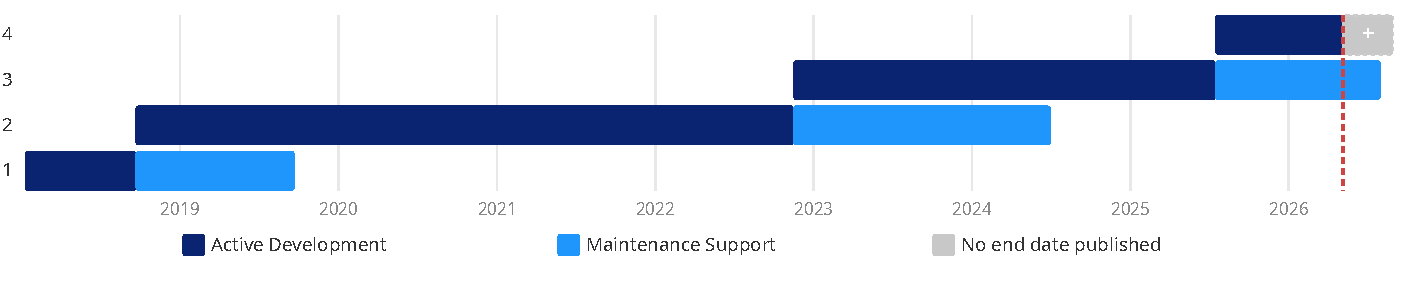
\includegraphics[width=\textwidth]{figures/nuxtoutdated.pdf}
\end{figure}

Eng damit verbunden ist die \emph{Failure Rate}: Das spaCy-Backend fehlt vollständig im Repository.
Die Prototyp-UI ist zwar lauffähig, erfordert jedoch einen manuellen Downgrade von Nuxt~3 auf Nuxt~2 sowie das separate Starten eines Docker-Containers für spaCy.
Das System ist nicht out-of-the-box reproduzierbar.

Hinsichtlich des \emph{Alters} ist der Prototyp differenziert zu bewerten.
Er wurde 2022 entwickelt, und der verwendete Stack war zum Zeitpunkt der Entwicklung aktuell -- Nuxt~2 befand sich bis November 2022 in aktiver Entwicklung~\cite{eol2026nuxt}.
Der Stack ist jedoch inzwischen veraltet, wie Abb.~\ref{fig:nuxt-eol} zeigt.

Die \emph{Performance} stellt kein Problem dar.
Die regelbasierte Analyse läuft clientseitig und verarbeitet Eingaben ohne wahrnehmbare Verzögerung; die spaCy-Tokenisierung benötigt für einzelne Sätze ebenfalls nur wenige Millisekunden.

Die \emph{Support Requirements} und \emph{Maintenance Costs} sind hingegen hoch.
Die Paketkonfiguration referenziert Nuxt~3, obwohl der Code Nuxt-2-APIs verwendet -- eine Inkonsistenz, die den Einstieg erschwert.
Das spaCy-Backend ist weder dokumentiert noch im Repository enthalten, es gibt weder CI/CD noch automatisierte Tests.
Die Abhängigkeiten können nicht aktualisiert werden, ohne Breaking Changes auszulösen, und eine inkrementelle Migration von Vue~2 auf Vue~3 ist aufgrund der fundamentalen API-Änderungen (Options API zu Composition API) nicht praktikabel.

Die \emph{Interoperability} ist neutral: Der Prototyp ist ein reiner Browser-Client ohne externe API; das spaCy-Backend stellt die einzige interne Schnittstelle dar.

\paragraph{Anwendungsbewertung.}

Die folgenden Befunde sind im Kontext eines Forschungsprototyps zu lesen, der als Proof-of-Concept konzipiert wurde und nicht den Anspruch produktionsreifer Software erhebt~\cite{loth2022masterprojekt}.

Die \emph{Understandability} der Codebasis ist eingeschränkt.
Zwar ist der Umfang mit wenigen Dateien überschaubar, doch die Hauptkomponente umfasst 1334~Zeilen und vermischt UI-Logik, NLP-Aufrufe, Verb-Matching, Scoring und Persistenz in einer einzigen Datei.
Variablennamen mischen Deutsch und Englisch; es finden sich Tippfehler in Bezeichnern und toter Code in Form leerer Methoden mit Alert-Aufrufen.

Die \emph{Documentation} beschränkt sich auf das DELFI-Paper~\cite{loth2022kompetenzeditor} und den zugehörigen Projektbericht~\cite{loth2022masterprojekt}.
Code-Dokumentation, Setup-Anleitung und API-Dokumentation für das spaCy-Backend fehlen vollständig.

Das \emph{Datenmodell} ist informell.
Das IndexedDB-Schema wird über Dexie implizit durch Seed-Daten in \texttt{db.js} definiert; alle Verblisten und Beispieltexte sind dort hardcodiert.
Die Verbliste enthält einen fehlerhaften Eintrag (\emph{Zusammenhänge} als Verb, obwohl es ein Nomen ist) sowie das Verb \emph{erkennen} in drei Taxonomiestufen ohne Disambiguierungslogik.

\emph{Performance} und \emph{Programmiersprache} sind unkritisch: JavaScript ist als Sprache aktuell und weit verbreitet; das Problem liegt nicht in der Sprache selbst, sondern in den veralteten Frameworks.

Das \emph{Configuration Management} weist die bereits genannte Inkonsistenz zwischen \texttt{package.json} und tatsächlich verwendeten APIs auf.
Es gibt kein CI/CD und keine Build-Pipeline.

Besonders gravierend ist das vollständige Fehlen von \emph{Test Data}: Es existieren keine automatisierten Tests, kein Test-Verzeichnis und kein Test-Framework in den Abhängigkeiten.

Der Original-Entwickler ist nicht am Projekt beteiligt; die Einarbeitung erfolgte durch Codeanalyse und die vorhandene Dokumentation.

\subsection{Funktionale Bewertung}\label{sec:funktionale-bewertung}

Der IST-SOLL-Abgleich stellt den aktuellen Zustand des Prototyps den definierten funktionalen und nicht-funktionalen Anforderungen gegenüber.
Tab.~\ref{tab:ist-soll} gibt eine kompakte Übersicht; die wesentlichen Befunde werden im Folgenden erläutert.

\begin{table}[H]
\caption{IST-SOLL-Abgleich: Erfüllungsstatus der Anforderungen\label{tab:ist-soll}}
\centering
\small
\begin{tabular}{llll}
\hline
\textbf{ID} & \textbf{Anforderung} & \textbf{Typ} & \textbf{Status} \\
\hline
FA1 & Klassifikation         & funktional       & teilweise erfüllt \\
FA2 & Taxonomie-Zuordnung    & funktional       & teilweise erfüllt \\
FA3 & Empfehlungen           & funktional       & teilweise erfüllt \\
FA4 & Set-Analyse            & funktional       & nicht erfüllt \\
FA5 & Echtzeit-Feedback      & funktional       & erfüllt \\
FA6 & Persistenz             & funktional       & teilweise erfüllt \\
\hline
NFA1 & Konfidenzmaße         & nicht-funktional & nicht erfüllt \\
NFA2 & Transparenz           & nicht-funktional & erfüllt \\
NFA3 & Deutsche Sprache      & nicht-funktional & erfüllt \\
NFA4 & Technologie-Migration & nicht-funktional & nicht erfüllt \\
NFA5 & Performance           & nicht-funktional & erfüllt \\
\hline
\end{tabular}
\end{table}

\paragraph{Erfüllte Anforderungen.}

Vier Anforderungen sind vollständig erfüllt und bilden die bewährten Stärken des Prototyps, die bei der Weiterentwicklung erhalten bleiben.
Das \emph{Echtzeit-Feedback} (FA5) funktioniert zuverlässig: Nach einer Tipp-Pause von 1000\,ms werden Verben farblich hervorgehoben -- grün für empfohlene, rot für nicht empfohlene, blau für NLP-erkannte und grau für nicht zugeordnete Verben.
Die \emph{Transparenz} (NFA2) ist eine besondere Stärke des regelbasierten Ansatzes: Jede Zuordnung ist direkt nachvollziehbar, da sie auf der Zugehörigkeit eines Verbs zu einer expliziten Liste basiert.
Info-Popups erklären die Bewertungslogik.
Die Unterstützung der \emph{deutschen Sprache} (NFA3) ist durch die deutsche Verbliste und das spaCy-Modell \texttt{de\_core\_news\_sm} gegeben.
Die \emph{Performance} (NFA5) ist durch die clientseitige Verarbeitung kleiner Datenmengen kein Problem.

\paragraph{Teilweise erfüllte Anforderungen.}

Die vier teilweise erfüllten Anforderungen bilden den Kern der vorliegenden Untersuchung.
In jedem Fall existiert ein funktionales Konzept im Prototyp, dessen Wirksamkeit jedoch durch die geschlossene Verbliste und die fehlende Nutzung der Taxonomie-Zuordnung begrenzt ist.

Bei der \emph{Klassifikation} (FA1) verfolgt der Prototyp einen impliziten Ansatz: Sätze ohne gelistetes Verb werden als \glqq entbehrlich\grqq\ markiert, was einer Nicht-Kompetenz-Klassifikation entspricht.
Dieses Konzept scheitert jedoch an Kompetenzformulierungen, die Verben verwenden, die nicht in der statischen Liste enthalten sind -- diese werden fälschlich als entbehrlich eingestuft.

Die \emph{Taxonomie-Zuordnung} (FA2) ist im Datenmodell angelegt: Die Verbliste in \texttt{db.js} enthält 80~Verben mit Zuordnung zu den sechs Stufen nach Anderson und Krathwohl~\cite{anderson2001taxonomy}.
Die Taxonomiestufe wird jedoch im UI nicht angezeigt; der Score ist rein binär (empfohlen/nicht empfohlen).
Darüber hinaus erscheint das Verb \emph{erkennen} in drei verschiedenen Stufen ohne Disambiguierungslogik.

Die \emph{Empfehlungsfunktion} (FA3) zeigt bei nicht empfohlenen Verben eine statische Tabelle aller empfohlenen Verben an -- immer dieselbe Liste, unabhängig vom Kontext des Satzes.
Eine ähnlichkeitsbasierte Auswahl findet nicht statt.

Die \emph{Persistenz} (FA6) unterstützt Speichern, Laden und Löschen über IndexedDB.
Die Speicherfunktion (\texttt{saveComp()}) verwendet jedoch ausschließlich \texttt{add()}, sodass jeder Speichervorgang einen neuen Eintrag erstellt, anstatt den bestehenden zu aktualisieren.

\paragraph{Nicht erfüllte Anforderungen.}

Drei Anforderungen sind nicht erfüllt.
Die \emph{Set-Analyse} (FA4) fehlt vollständig: Der Prototyp analysiert jeden Satz einzeln; es gibt keine Aggregation auf Modulebene, keine Taxonomie-Verteilung und keine Abdeckungsanalyse.
\emph{Konfidenzmaße} (NFA1) existieren nicht -- der vorhandene Score ist ein Gesamt-Qualitätsprozentsatz für den gesamten Text, kein Konfidenzwert pro Zuordnung.
Die \emph{Technologie-Migration} (NFA4) steht aus: Der gesamte Stack (Nuxt~2, Vue~2, Vuetify~2) ist End-of-Life.

\paragraph{Selbstidentifizierte Limitationen.}

Loth und Konert benennen in ihrem Fazit selbst Erweiterungswünsche, die den hier identifizierten Lücken entsprechen~\cite{loth2022kompetenzeditor,loth2022masterprojekt}.
Die Autoren fordern, dass \glqq Schlüsselwörter auch in abgewandelter, konjugierter und weiterer abweichender Form von der Software analysiert werden können\grqq~\cite{loth2022kompetenzeditor} -- eine Fähigkeit, die ein Embedding-basierter Ansatz prinzipbedingt mitbringt, da er nicht auf exakte Zeichenketten, sondern auf semantische Ähnlichkeit operiert.
Darüber hinaus identifizieren die Autoren die Möglichkeit, Texte \glqq in eine weitere Datenbank gespeist werden und mit anderen Kompetenzen dieser Domäne verglichen oder automatisch um Vorschläge aus anderen Texten ergänzt werden\grqq~\cite{loth2022kompetenzeditor} zu lassen -- dies entspricht der ähnlichkeitsbasierten Empfehlungsfunktion (FA3).
Schließlich weisen die Autoren auf die fehlende formale Evaluation hin, die durch den in dieser Arbeit erstellten Gold-Standard-Datensatz adressiert wird.

\subsection{Strategische Einordnung}\label{sec:strategische-einordnung}

Sommerville~\cite{sommerville2016software} unterscheidet vier strategische Optionen für den Umgang mit Legacy-Systemen, basierend auf einer kombinierten Bewertung von Geschäftswert und technischer Qualität:
Abschalten (\emph{Scrap}), Weiterbetreiben (\emph{Maintain}), Modernisieren (\emph{Reengineer}) oder Ersetzen (\emph{Replace}).

Der Prototyp weist einen \textbf{hohen konzeptionellen Wert} auf: Das Konzept wurde publiziert~\cite{loth2022kompetenzeditor}, die regelbasierte Analyse funktioniert zuverlässig für gelistete Verben, und vier der elf Anforderungen sind bereits erfüllt (vgl. Tab.~\ref{tab:ist-soll}).
Gleichzeitig ist die \textbf{technische Qualität niedrig}: Der Stack ist veraltet, es gibt keine automatisierten Tests, die Code-Dokumentation fehlt und die fehlende Trennung von Verantwortlichkeiten erschwert gezielte Änderungen.

Diese Kombination -- hoher Geschäftswert bei niedriger technischer Qualität -- entspricht in Sommervilles Bewertungsmatrix (Figure~9.9) dem Cluster \emph{Low quality, high business value}, für das Reengineering empfohlen wird~\cite{sommerville2016software}.
Ein Abschalten scheidet aufgrund des bewährten Konzepts aus; ein bloßes Weiterbetreiben ist nicht möglich, da die Abhängigkeiten keine Security-Patches mehr erhalten; eine vollständige Neuentwicklung wäre unverhältnismäßig, da Architektur und UI-Konzepte wiederverwendbar sind.

Die Weiterentwicklung lässt sich als Kombination zweier Wartungstypen einordnen:
\emph{Environmental Adaptation} -- die Migration des Frameworks von Nuxt~2 auf Nuxt~4 und von Vue~2 auf Vue~3 -- sowie \emph{Functionality Addition} -- die Integration der Embedding-basierten Analysefunktionen.
Dabei wird die Architektur des Prototyps beibehalten, der Quellcode jedoch aufgrund der umfangreichen Breaking Changes zwischen den Framework-Versionen weitgehend überarbeitet.


\section{Systementwurf}\label{sec:entwurf}
% =============================================================================
% Kapitel 5: Systementwurf
% =============================================================================

Aufbauend auf der Analyse des bestehenden Systems (Kap.~\ref{sec:vorarbeit}) und den definierten Anforderungen (Kap.~\ref{sec:anforderungen}) wird in diesem Kapitel der Entwurf des erweiterten Systems dargelegt.
Dabei wird zunächst die Gesamtarchitektur beschrieben, anschließend das hybride Cascading-Muster im Detail erläutert und abschließend die wesentlichen Technologieentscheidungen begründet.

\subsection{Gesamtarchitektur}\label{sec:architektur}

Die Architekturentscheidung ergibt sich aus zwei Randbedingungen: Erstens erfordert das gewählte Sentence-Embedding-Modell mit 278 Millionen Parametern eine serverseitige Inferenz -- eine Ausführung im Browser ist aufgrund der Modellgröße und des Speicherbedarfs nicht praktikabel.
Zweitens sollen die trainierten SVM-Klassifikatoren und die Referenzdatenbank zentral vorgehalten werden, um konsistente Analyseergebnisse zu gewährleisten.
Daraus resultiert eine Zwei-Komponenten-Architektur aus einem Browser-Frontend und einem Python-Backend, die über eine REST-API kommunizieren.

Abb.~\ref{fig:architektur-gesamt} zeigt die Gesamtarchitektur.
Das \textbf{Frontend} ist eine Single-Page-Application auf Basis von Nuxt~4 und Vue~3.
Es besteht aus drei Hauptbereichen: dem Tiptap-Editor mit Echtzeit-Verb-Highlighting, einem Analyse-Panel, das pro Satz Typ, Taxonomiestufe, Konfidenz und Quelle anzeigt, sowie einer Set-Analyse-Übersicht, die die Taxonomie-Verteilung auf Modulebene darstellt.
Bei jeder Texteingabe sendet das Frontend nach einer Debounce-Pause den vollständigen Text über die REST-API an das Backend.

Das \textbf{Backend} ist ein Python-Service auf Basis von FastAPI.
Es stellt einen einzigen Analyse-Endpunkt bereit (\texttt{POST /api/analyze}), der den Eingabetext entgegennimmt und ein strukturiertes Ergebnis zurückgibt.
Intern orchestriert eine Hybrid-Analyse-Pipeline sechs Verarbeitungsschritte (vgl. Kap.~\ref{sec:cascading-entwurf}).
Beim Start des Services werden alle benötigten Modelle und Daten in den Speicher geladen: das SBERT-Modell für die Embedding-Berechnung, die beiden SVM-Klassifikatoren für Typ- und Taxonomie-Zuordnung, die vorberechneten Referenz-Embeddings sowie das spaCy-Modell für linguistische Vorverarbeitung.

\begin{figure}[t!]
\caption{Gesamtarchitektur des Systems. Das Frontend kommuniziert über eine REST-API mit dem Backend, das die Hybrid-Analyse-Pipeline, trainierte Modelle und die Referenzdatenbank kapselt.\label{fig:architektur-gesamt}}
\centering
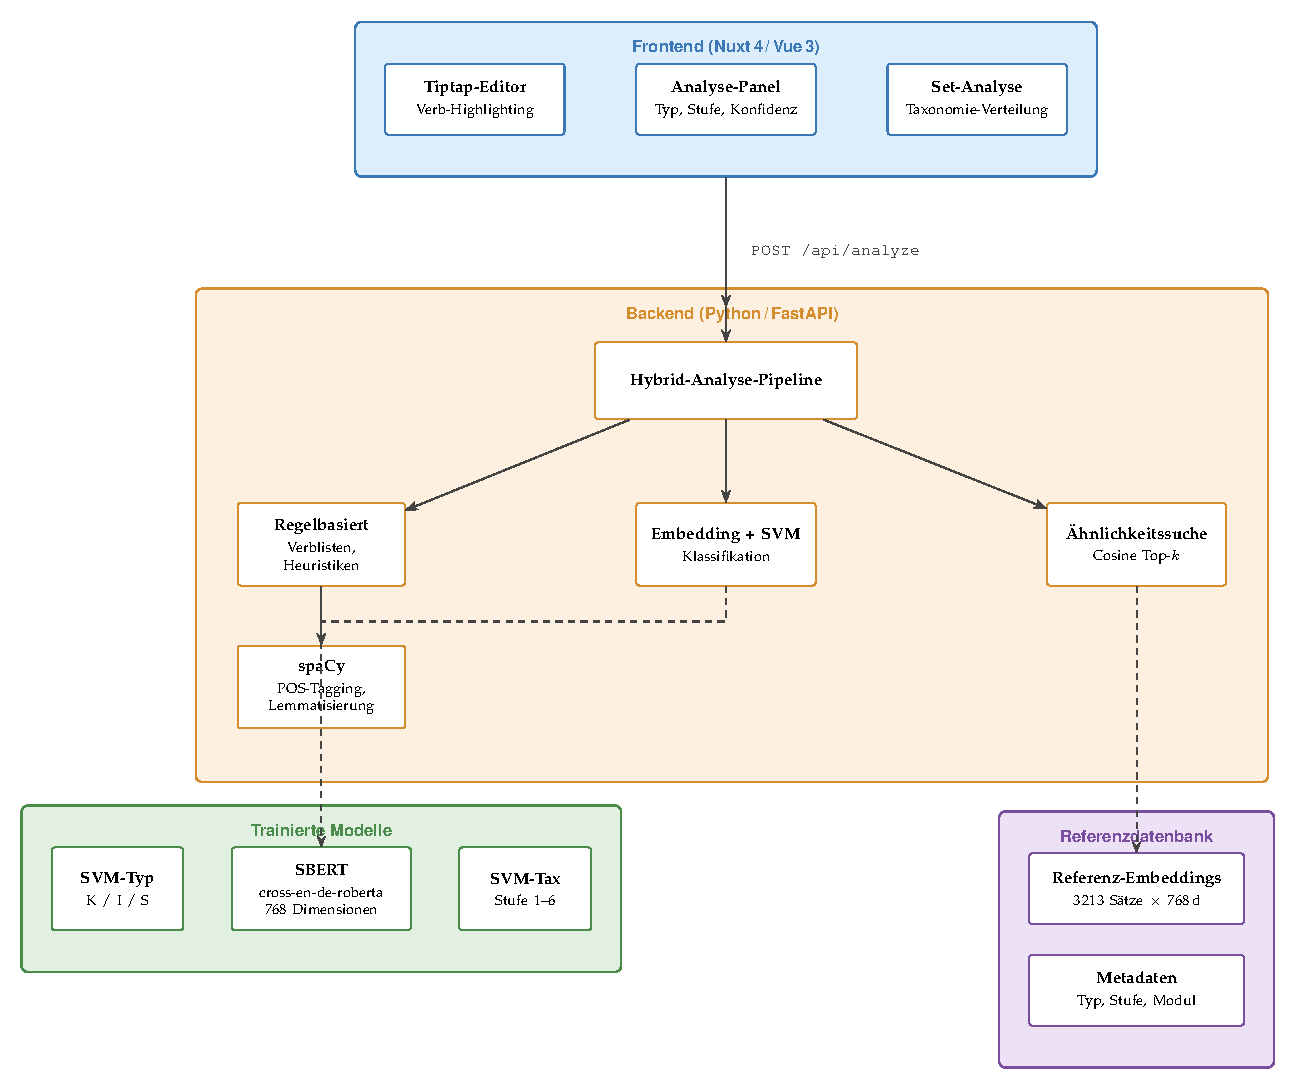
\includegraphics[width=\textwidth]{figures/architektur_gesamt.pdf}
\end{figure}

Die Schnittstelle zwischen Frontend und Backend ist bewusst minimal gehalten: Ein einzelner Endpunkt nimmt den Text entgegen und liefert alle Analyseergebnisse -- Satztyp, Taxonomiestufe, Konfidenz, erkannte Verben, ähnliche Formulierungen und Set-Analyse -- in einer JSON-Antwort zurück.
Diese Bündelung vermeidet mehrfache Roundtrips und vereinfacht die Frontend-Logik, da keine Zustandssynchronisation zwischen verschiedenen API-Aufrufen erforderlich ist.

Ergänzend stellt ein Health-Endpunkt (\texttt{GET /api/health}) den Ladestatus der Modelle bereit, sodass das Frontend den Systemzustand anzeigen kann.

\subsection{Hybrid-Cascading-Entwurf}\label{sec:cascading-entwurf}

Der Kern des Systems ist eine hybride Pipeline, die regelbasierte und Embedding-basierte Analyse in einem Cascading-Muster kombiniert.
Die Leitidee ist, für eindeutige Fälle die transparente und schnelle regelbasierte Zuordnung zu nutzen und nur für mehrdeutige oder unbekannte Fälle auf die kontextsensitive Embedding-Klassifikation zurückzugreifen.
Abb.~\ref{fig:cascading} zeigt den Ablauf.

\begin{figure}[t!]
\caption{Hybrid-Cascading-Pipeline. Regelbasierte Zuordnung greift bei eindeutigen Verben; bei mehrdeutigen oder unbekannten Verben wird die Embedding-basierte Klassifikation als Fallback eingesetzt.\label{fig:cascading}}
\centering
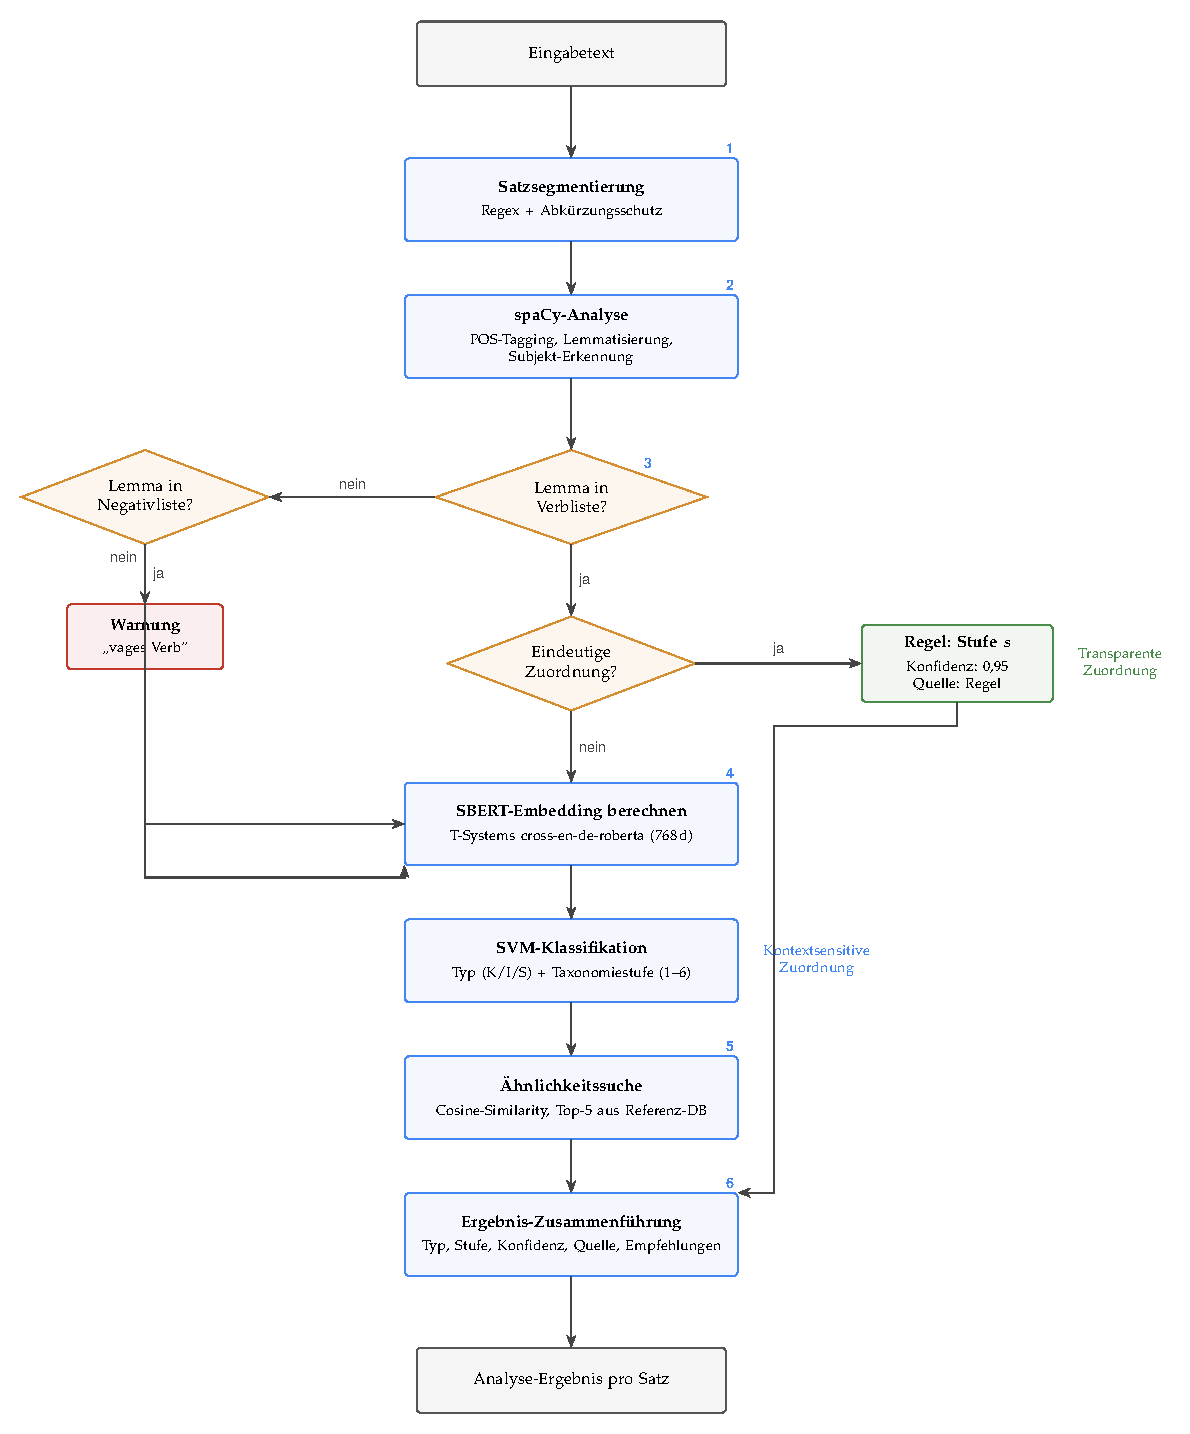
\includegraphics[width=0.72\textwidth]{figures/architektur_cascading.pdf}
\end{figure}

\subsubsection{Schritt 1: Satzsegmentierung}\label{sec:segmentierung}

Der Eingabetext wird in einzelne Sätze aufgeteilt.
Die Segmentierung verwendet spaCy, ergänzt um Schutzmechanismen für Abkürzungen (z.\,B., bzw., Prof., Dr.), die andernfalls zu falschen Satzgrenzen führen würden.
Aufzählungen und Infinitivkonstruktionen mit Semikolon werden als zusammengehörig behandelt.

\subsubsection{Schritt 2: Linguistische Vorverarbeitung}\label{sec:spacy-analyse}

Jeder Satz wird mit dem spaCy-Modell \texttt{de\_core\_news\_lg} analysiert.
Die Verarbeitung umfasst drei Aspekte: POS-Tagging zur Identifikation von Verben, Lemmatisierung zur Reduktion auf die Grundform und Subjekt-Erkennung zur Prüfung, ob \emph{die Studierenden} als Subjekt auftreten -- ein Indikator für eine Kompetenzformulierung.

\subsubsection{Schritt 3: Regelbasierte Klassifikation}\label{sec:regelbasiert}

Die regelbasierte Klassifikation operiert auf den extrahierten Verb-Lemmata und prüft diese gegen drei Listen: eine Positivliste empfohlener Verben mit Taxonomie-Zuordnung, eine Negativliste nicht empfohlener Verben und eine Liste von Modalverben.

Die Entscheidungslogik folgt einem kaskadierenden Schema.
Zunächst wird der \emph{Satztyp} bestimmt: Enthält der Satz ein erkanntes Subjekt (\emph{Studierende}) und mindestens ein Verb, wird er als Kompetenzformulierung (K) eingestuft; enthält er weder ein solches Subjekt noch ein Handlungsverb, wird er als Inhaltsbeschreibung (I) oder sonstiger Satz (S) klassifiziert.

Für als K klassifizierte Sätze wird anschließend die \emph{Taxonomiestufe} bestimmt.
Befindet sich das Lemma des Hauptverbs in der Positivliste und ist dort genau einer Stufe zugeordnet, wird diese Stufe direkt übernommen -- mit einer Konfidenz von 0{,}95 und der Quellenangabe \emph{Regel}.
Dieser Fall bildet den \emph{Short Circuit} des Cascading-Musters: Die Zuordnung ist abgeschlossen, ohne dass Embeddings berechnet werden müssen.

Ist das Verb zwar gelistet, aber mehreren Stufen zugeordnet (z.\,B. \emph{erkennen} auf Stufe~1, 2 und~4), oder befindet es sich nicht in der Positivliste, wird die Analyse an Schritt~4 delegiert.
Befindet sich das Verb in der Negativliste, wird zusätzlich eine Warnung erzeugt, die den Nutzenden auf die Verwendung eines unspezifischen Verbs hinweist.

\subsubsection{Schritt 4: Embedding-basierte Klassifikation}\label{sec:embedding-klassifikation}

Für alle Sätze, bei denen die regelbasierte Stufe keine eindeutige Zuordnung liefert, wird der vollständige Satz durch das SBERT-Modell in einen 768-dimensionalen Vektor überführt.
Auf diesem Embedding operieren zwei SVM-Klassifikatoren:

Der \emph{Typ-Klassifikator} ordnet den Satz den Klassen K, I oder S zu.
Er greift nur, wenn Schritt~3 keine eindeutige Typ-Bestimmung ergeben hat -- etwa bei Sätzen ohne erkanntes Subjekt, die dennoch Kompetenzformulierungen sein können (z.\,B. Passivkonstruktionen).

Der \emph{Taxonomie-Klassifikator} ordnet Kompetenzformulierungen einer der sechs Stufen nach Anderson und Krathwohl zu.
Er berücksichtigt den gesamten Satzkontext, nicht nur das isolierte Verb.
Dadurch kann er auch Verben korrekt einordnen, die je nach Kontext unterschiedlichen Stufen angehören -- eine Fähigkeit, die der regelbasierten Analyse prinzipbedingt fehlt.

Beide Klassifikatoren geben neben der Vorhersage eine Konfidenz aus, die aus der Wahrscheinlichkeitsschätzung der SVM (\texttt{predict\_proba}) abgeleitet wird.
Die Quellenangabe wechselt auf \emph{Embedding}.

\subsubsection{Schritt 5: Ähnlichkeitssuche}\label{sec:aehnlichkeitssuche}

Unabhängig von der Cascading-Entscheidung wird für jeden als Kompetenzformulierung klassifizierten Satz eine Ähnlichkeitssuche durchgeführt.
Das in Schritt~4 berechnete Embedding -- oder, falls der Satz bereits in Schritt~3 abgeschlossen wurde, ein nachträglich berechnetes Embedding -- wird gegen die Referenzdatenbank verglichen (vgl. Kap.~\ref{sec:referenz-db}).

Die Suche berechnet die Cosine-Similarity zwischen dem Eingabe-Embedding und allen Referenz-Embeddings und gibt die fünf ähnlichsten Formulierungen zurück, sortiert nach Similarity.
Für jede Empfehlung werden der Satztext, die Taxonomiestufe, der Similarity-Wert und die Herkunft (Modulname, Studiengang) angegeben.

\subsubsection{Schritt 6: Ergebnis-Zusammenführung}\label{sec:zusammenfuehrung}

Im letzten Schritt werden die Einzelergebnisse zu einem strukturierten Analyseergebnis pro Satz zusammengeführt.
Dieses enthält den Satztyp (K/I/S), die Taxonomiestufe (1--6 oder null), die Konfidenz (0--1), die Quelle (Regel oder Embedding), die erkannten Verben mit ihren Kategorien und Hervorhebungsklassen, die fünf ähnlichsten Referenzformulierungen sowie etwaige Warnungen.

Zusätzlich wird auf Textebene eine \emph{Set-Analyse} berechnet: Die Taxonomiestufen aller Kompetenzformulierungen werden aggregiert, die Abdeckung (Anzahl belegter Stufen) ermittelt und eine textuelle Empfehlung für fehlende Stufen generiert.
Diese Aggregation adressiert die Anforderung FA4 (Set-Analyse auf Modulebene).

\subsubsection{Cascading-Effizienz}\label{sec:cascading-effizienz}

Vom Cascading-Muster werden zwei Vorteile erwartet, die in Kap.~\ref{sec:kosten-nutzen} empirisch überprüft werden.
Erstens \emph{Transparenz}: Für Verben, die eindeutig in der Positivliste stehen, ist die Zuordnung direkt nachvollziehbar -- sie basiert auf einer expliziten Listenregel, nicht auf einer Blackbox-Klassifikation.
Die Quellenangabe (Regel vs. Embedding) macht für jeden Satz transparent, welches Verfahren die Zuordnung vorgenommen hat (NFA2).

Zweitens \emph{Performance}: Die regelbasierte Prüfung ist ein Dictionary-Lookup und benötigt unter 1\,ms.
Nur wenn dieser Lookup keine eindeutige Zuordnung liefert, wird die rechenintensivere Embedding-Berechnung ausgelöst.
Die Erwartung ist, dass Modulhandbücher überwiegend Standardverben enthalten und ein Großteil der Sätze den Short Circuit nutzen kann.
Tab.~\ref{tab:performance} zeigt die gemessenen Verarbeitungszeiten.

\begin{table}[H]
\caption{Verarbeitungszeiten der Pipeline-Schritte auf CPU\label{tab:performance}}
\centering
\small
\begin{tabular}{lrl}
\hline
\textbf{Schritt} & \textbf{Zeit} & \textbf{Anmerkung} \\
\hline
Satzsegmentierung & $<$\,1\,ms & Regex \\
spaCy POS-Tagging & $\sim$\,5\,ms/Satz & de\_core\_news\_lg \\
Regelbasierter Check & $<$\,1\,ms & Dictionary-Lookup \\
SBERT Encoding & $\sim$\,2\,ms/Satz & 546 Sätze/s (CPU) \\
SVM-Klassifikation & $<$\,1\,ms & Trainierte sklearn-Pipeline \\
Cosine-Similarity & $\sim$\,1\,ms & NumPy-Dot-Produkt \\
\hline
\textbf{Gesamt pro Satz} & $\sim$\,\textbf{10\,ms} & \\
\textbf{Typischer Modultext (5--10 Sätze)} & $\sim$\,\textbf{50--100\,ms} & Unter NFA5 ($<$\,2\,s) \\
\hline
\end{tabular}
\end{table}

\subsection{Modellauswahl}\label{sec:modellauswahl}

Die Wahl des Sentence-Embedding-Modells bestimmt maßgeblich die Klassifikationsleistung des Embedding-basierten Pfads.
Drei Kandidaten wurden systematisch evaluiert, die unterschiedliche Kompromisse zwischen Dimensionalität, Geschwindigkeit und Genauigkeit repräsentieren.

\subsubsection{Evaluierte Modelle}\label{sec:eval-modelle}

Alle drei Modelle sind vortrainierte Sentence-Transformer, die über die Hugging-Face-Plattform verfügbar sind und deutsche Texte unterstützen:

\begin{itemize}
  \item \textbf{paraphrase-multilingual-MiniLM-L12-v2} (384\,d): Ein kompaktes multilinguales Modell mit hoher Inferenzgeschwindigkeit (1\,859 Sätze/s), das durch Knowledge Distillation aus einem größeren Modell gewonnen wurde~\cite{reimers2020multilingual}.
  \item \textbf{deutsche-telekom/gbert-large-paraphrase-cosine} (1\,024\,d): Ein auf deutschem Text vortrainiertes BERT-Large-Modell mit der höchsten Dimensionalität, aber geringster Geschwindigkeit (203 Sätze/s).
  \item \textbf{T-Systems-onsite/cross-en-de-roberta-sentence-transformer} (768\,d): Ein cross-linguales RoBERTa-Modell, das auf englisch-deutschen Paraphrasen-Daten feinabgestimmt wurde und von der Reichhaltigkeit englischer Trainingskorpora profitiert.
\end{itemize}

\subsubsection{Evaluationsmethodik}\label{sec:eval-methodik-modelle}

Die Modellauswahl erfolgte auf dem initialen Datensatz der Hochschule Fulda (3\,213 Sätze, 80/20-Split, Seed~42), der zum Zeitpunkt der Entwurfsentscheidung vorlag.
Die finale Evaluation auf dem erweiterten, multiuniversitären Datensatz folgt in Kap.~\ref{sec:evaluation}.
Für jedes Modell wurde derselbe Klassifikator trainiert: eine SVM mit RBF-Kernel (C\,=\,10, gamma\,=\,scale) nach Standardisierung der Features (StandardScaler).
Die Hyperparameter wurden nicht optimiert, um einen fairen Vergleich der Embedding-Qualität -- unabhängig von Klassifikator-Tuning -- zu ermöglichen.
Als Metrik dient der gewichtete F1-Score auf dem Test-Split (641 Sätze).

\subsubsection{Ergebnisse und Entscheidung}\label{sec:modell-entscheidung}

Tab.~\ref{tab:modellvergleich} zeigt die Ergebnisse.

\begin{table}[H]
\caption{Vergleich der evaluierten Sentence-Embedding-Modelle\label{tab:modellvergleich}}
\centering
\small
\begin{tabular}{lrrrr}
\hline
\textbf{Modell} & \textbf{Dim} & \textbf{Sätze/s} & \textbf{Typ-F1} & \textbf{Tax-F1} \\
\hline
MiniLM-L12-v2 & 384 & 1\,859 & 0{,}977 & 0{,}846 \\
gbert-large & 1\,024 & 203 & 0{,}979 & 0{,}875 \\
\textbf{cross-en-de-roberta} & \textbf{768} & \textbf{546} & \textbf{0{,}977} & \textbf{0{,}906} \\
\hline
\end{tabular}
\end{table}

Alle drei Modelle erzielen bei der Typ-Klassifikation (K/I/S) nahezu identische Ergebnisse (F1 $\geq$ 0{,}977), was darauf hindeutet, dass die Unterscheidung zwischen Kompetenzformulierungen und Inhaltsbeschreibungen eine vergleichsweise einfache Aufgabe darstellt.
Die entscheidende Differenzierung zeigt sich bei der Taxonomie-Klassifikation: Hier übertrifft das cross-en-de-roberta-Modell von T-Systems das gbert-large-Modell um 3{,}1 Prozentpunkte und das MiniLM-Modell um 6{,}0 Prozentpunkte.

Das \textbf{T-Systems-onsite/cross-en-de-roberta-sentence-transformer} wird gewählt.
Die Entscheidung basiert auf drei Faktoren: (1)~die beste Taxonomie-Klassifikation (F1\,=\,0{,}906), die für die Kernfunktionalität des Systems ausschlaggebend ist; (2)~ein guter Kompromiss bei der Geschwindigkeit (546 Sätze/s -- 2{,}7$\times$ schneller als gbert-large); (3)~eine mittlere Dimensionalität (768\,d), die einen Kompromiss zwischen semantischer Ausdruckskraft und Speicherbedarf für die Ähnlichkeitssuche darstellt.

\subsubsection{SVM-Klassifikator-Architektur}\label{sec:svm-architektur}

Für beide Klassifikationsaufgaben wird eine sklearn-Pipeline aus StandardScaler und SVC mit RBF-Kernel eingesetzt.
Die Wahl der SVM folgt Kumar et al.~\cite{kumar2025automated}, die auf einem vergleichbaren Datensatz (Bloom-Taxonomie-Klassifikation englischer Lernergebnisse) zeigen, dass eine SVM auf Embeddings (94\,\% Accuracy) alle evaluierten Deep-Learning-Modelle übertrifft.
Die RBF-SVM ermöglicht durch die Kernelfunktion eine nichtlineare Entscheidungsgrenze im Embedding-Raum und gibt über die Platt-Skalierung (\texttt{probability=True}) kalibrierte Konfidenzwerte aus, die als Grundlage für die Konfidenzanzeige im Frontend dienen (NFA1).

Auf dem initialen Fulda-Datensatz (641~Test-Sätze) erreicht der Typ-Klassifikator (K/I/S) einen gewichteten F1-Score von 0{,}977 und der Taxonomie-Klassifikator (Stufen 1--6, nur K-Sätze) einen gewichteten F1-Score von 0{,}906.
Diese Werte dienen als Entwurfsgrundlage; die detaillierte Auswertung auf dem erweiterten Datensatz erfolgt in Kap.~\ref{sec:evaluation}.

\subsection{Referenzdatenbank}\label{sec:referenz-db}

Die Referenzdatenbank dient als Grundlage für die ähnlichkeitsbasierte Empfehlungsfunktion (FA3).
Sie enthält vorberechnete Embeddings aller Sätze aus dem Gold-Standard-Datensatz und ermöglicht eine effiziente Suche nach semantisch ähnlichen Formulierungen.

\subsubsection{Aufbau}

Die Datenbank besteht aus zwei Komponenten: einer Matrix normalisierter 768-dimensionaler Embedding-Vektoren (\texttt{.npy}-Datei) und einer JSON-Metadatendatei, die pro Satz den Text, den Satztyp, die Taxonomiestufe, den Modulnamen und den Studiengang speichert.
Die Embeddings werden mit demselben SBERT-Modell berechnet, das auch zur Laufzeit für Eingabesätze verwendet wird, um eine konsistente Repräsentation zu gewährleisten.

Die Normalisierung der Embedding-Vektoren auf Einheitslänge ist eine bewusste Entwurfsentscheidung: Für normalisierte Vektoren reduziert sich die Cosine-Similarity auf ein Dot-Produkt, das mit NumPy als Matrix-Vektor-Multiplikation in unter 1\,ms berechenbar ist.
Damit kann die Suche über alle Referenzen zur Laufzeit durchgeführt werden, ohne dass ein Approximate-Nearest-Neighbor-Index erforderlich wäre.

\subsubsection{Datengrundlage}

Die Referenzdatenbank wird aus dem Gold-Standard-Datensatz (vgl. Kap.~\ref{sec:eval-goldstandard}) aufgebaut, der über 5\,600~Sätze aus Modulhandbüchern von vier Hochschulen und vier Fachbereichen umfasst.
Die Annotation (Satztyp, Taxonomiestufe und Formulierungsqualität) erfolgte LLM-gestützt und wurde manuell validiert (vgl. Kap.~\ref{sec:eval-vorannotation}).
Die Referenzdatenbank nutzt den gesamten Datensatz -- nicht nur den Trainings-Split --, da bei der Ähnlichkeitssuche kein Klassifikator trainiert wird und somit kein Overfitting-Risiko besteht.
Durch die Einbeziehung externer Hochschulen deckt die Referenzdatenbank ein breiteres Spektrum an Formulierungsstilen ab und ermöglicht domänenübergreifende Empfehlungen.


\section{Implementierung}\label{sec:implementierung}
% =============================================================================
% Kapitel 6: Implementierung
% =============================================================================

Dieses Kapitel beschreibt die technische Umsetzung des in Kap.~\ref{sec:entwurf} entworfenen Systems.
Zunächst wird die Framework-Migration behandelt, anschließend die Integration der Embedding-basierten Analysefunktionen und abschließend die Gestaltung der Benutzeroberfläche.

\subsection{Framework-Migration}\label{sec:migration}

Die in Kap.~\ref{sec:vorarbeit} identifizierten Defizite lassen sich in zwei Kategorien einteilen: technische Defizite, die durch die Framework-Migration adressiert werden, und funktionale Lücken, die durch die Embedding-basierte Erweiterung geschlossen werden sollen.
Dieser Abschnitt beschreibt die Migrationsentscheidungen; die Embedding-Integration folgt in Kap.~\ref{sec:impl-embedding}.

\subsubsection{Technologieentscheidungen}\label{sec:tech-entscheidungen}

Die fehlende Supplier Stability (NFA4) erfordert die Migration der drei zentralen Abhängigkeiten: Nuxt~2 wird durch Nuxt~4, Vue~2 durch Vue~3 und Vuetify~2 durch Vuetify~4 ersetzt.
Damit werden ausschließlich aktiv gewartete Frameworks eingesetzt, die Security-Patches und langfristigen Support erhalten.

Der in der Anwendungsbewertung kritisierte Mangel an Separation of Concerns -- die gesamte Anwendungslogik in einer 1334-zeiligen Datei -- wird durch den Wechsel von der Options API auf die Composition API adressiert.
Vue~3 erlaubt es, zusammengehörige Logik in sogenannte Composables zu extrahieren, anstatt sie nach Optionstyp (\texttt{data}, \texttt{methods}, \texttt{computed}) zu gruppieren.
Dadurch wird die monolithische Editorkomponente in spezialisierte Module aufgeteilt.

Die von Loth und Konert selbst identifizierte Limitation~L1 -- die fehlerhafte Texthervorhebung im Volltexteditor~\cite{loth2022kompetenzeditor} -- wird durch den Ersatz der ContentEditable-Komponente durch Tiptap~3 adressiert.
Der Prototyp verwendete die Browser-API \texttt{ContentEditable} direkt, was dazu führte, dass HTML-Manipulation und Cursorposition manuell synchronisiert werden mussten.
Tiptap basiert auf ProseMirror und arbeitet mit einem strukturierten Dokumentenmodell, in dem Textmarkierungen deklarativ als sogenannte Marks definiert werden.
Die Farbcodierung der Verben wird über Custom Marks realisiert, die den vier Kategorien des Prototyps entsprechen: empfohlen, nicht empfohlen, NLP-erkannt und nicht zugeordnet.

Das inkonsistente Configuration Management wird durch den Wechsel von Vuex auf Pinia sowie durch den Einsatz auto-importierter Composables anstelle globaler Plugins vereinheitlicht.
Das informelle Datenmodell -- im Prototyp als hardcodierte Seed-Daten in einer Plugin-Datei realisiert -- wird in ein separates Datenmodul überführt, das ein explizites Schema definiert.
Die Datenbankschicht nutzt Dexie~4 und kapselt alle Verblisten, Taxonomie-Zuordnungen und CRUD-Operationen.

\subsubsection{Architektur der migrierten Anwendung}\label{sec:architektur-migration}

Kern der Restrukturierung ist die Aufteilung der Editorkomponente in vier Composables, die jeweils eine abgegrenzte Verantwortlichkeit übernehmen.
Das Composable \texttt{useDatabase} kapselt die Dexie-Anbindung und stellt Verblisten, Persistenz und CRUD-Operationen bereit; es adressiert den Befund des informellen Datenmodells, indem das Schema explizit definiert wird.
\texttt{useVerbAnalysis} enthält die Kernlogik der regelbasierten Analyse: Verb-Extraktion, Abgleich mit der Verbliste und Farbzuordnung -- Funktionalität, die im Prototyp über mehrere Methoden verteilt war.
\texttt{useSpacy} isoliert die Kommunikation mit dem spaCy-Backend für POS-Tagging als eigenständige Abhängigkeit, sodass diese Schnittstelle später durch das Embedding-Backend ersetzt werden kann.
\texttt{useScoring} extrahiert die Berechnung des Qualitäts-Scores, die im Prototyp in die UI-Komponente eingebettet war.

Die Seitenkomponente selbst beschränkt sich auf Template und UI-Steuerung; die fachliche Logik wird vollständig über die Composables bezogen.

\subsubsection{Erhaltene Funktionalität}\label{sec:erhaltene-funktionalitaet}

Die Migration verfolgt das Ziel, die in Tab.~\ref{tab:ist-soll} als erfüllt bewerteten Anforderungen zu erhalten.
Das Echtzeit-Feedback (FA5) wird durch denselben Debounce-Mechanismus realisiert -- nach einer Tipp-Pause wird die Analyse angestoßen und das Ergebnis als farbliche Hervorhebung im Editor dargestellt.
Die Transparenz (NFA2) bleibt durch die regelbasierte Zuordnung gewährleistet, die deutsche Sprachunterstützung (NFA3) durch die unveränderte Verbliste und das spaCy-Modell sichergestellt, und die Performance (NFA5) durch die weiterhin clientseitige regelbasierte Analyse gegeben.

Die Persistenz (FA6) wird gegenüber dem Prototyp verbessert: Die Speicherfunktion unterscheidet nun zwischen Neuanlage und Aktualisierung bestehender Einträge und adressiert damit den in der IST-Analyse dokumentierten Fehler, bei dem jeder Speichervorgang einen neuen Eintrag erstellte.

\subsubsection{Reproduzierbarkeit und Orchestrierung}\label{sec:orchestrierung}

Die IST-Analyse identifizierte zwei zusammenhängende Defizite: Das spaCy-Backend fehlt im Repository, und das System ist nicht out-of-the-box reproduzierbar (vgl. Kap.~\ref{sec:technische-bewertung}, Failure Rate).
Beide Defizite werden durch eine Docker-Compose-Konfiguration adressiert, die das spaCy-Backend als Container bereitstellt.
Ein einzelner Befehl startet sowohl das NLP-Backend als auch den Entwicklungsserver der Anwendung; die manuelle Einrichtung separater Dienste entfällt damit.
Die Nuxt-Konfiguration leitet API-Anfragen über einen Proxy an den spaCy-Container weiter, sodass Frontend und Backend ohne manuelle URL-Konfiguration zusammenarbeiten.

Das in der IST-Analyse festgestellte Fehlen von CI/CD und automatisierten Tests (vgl. Kap.~\ref{sec:technische-bewertung}, Configuration Management) wird im Rahmen dieser Arbeit nicht vollständig adressiert, da der Fokus auf der Embedding-basierten Analysefunktionalität liegt.
Die Architekturentscheidung für isolierte Composables schafft jedoch die Voraussetzung für eine spätere Testbarkeit: Jedes Composable kann unabhängig von der UI-Schicht getestet werden.

\subsection{Embedding-Integration}\label{sec:impl-embedding}

Die in Kap.~\ref{sec:entwurf} entworfene Hybrid-Pipeline wird als Python-Backend realisiert, das drei Dienste kapselt: die Analyse-Pipeline, den Embedding-Service und die Ähnlichkeitssuche.
Dieser Abschnitt beschreibt die Implementierung dieser Komponenten.

\subsubsection{Backend-Service}\label{sec:backend-service}

Der Backend-Service nutzt FastAPI mit dem Lifespan-Pattern: Beim Serverstart werden alle Modelle und Daten synchron in den Speicher geladen, bevor der erste Request bearbeitet wird.
Das spaCy-Modell \texttt{de\_core\_news\_lg}, das SBERT-Modell, die beiden SVM-Klassifikatoren und die Referenz-Embeddings stehen anschließend für die gesamte Laufzeit im Speicher bereit.

Die API ist bewusst auf zwei Endpunkte beschränkt.
Der Health-Endpunkt (\texttt{GET /health}) gibt den Ladestatus der Modelle zurück, sodass das Frontend prüfen kann, ob das Backend betriebsbereit ist.
Der Analyse-Endpunkt (\texttt{POST /analyze}) nimmt den Eingabetext entgegen, delegiert die Verarbeitung an die Pipeline und gibt das strukturierte Ergebnis zurück.
CORS ist für die Entwicklungsumgebung offen konfiguriert; die Nuxt-Konfiguration leitet API-Anfragen über einen Proxy an den Backend-Service weiter, sodass Frontend und Backend unter derselben Origin operieren.

\subsubsection{Analyse-Pipeline}\label{sec:impl-pipeline}

Die Klasse \texttt{AnalysisPipeline} orchestriert die sechs Verarbeitungsschritte aus Kap.~\ref{sec:cascading-entwurf}.
Sie kapselt die Abhängigkeiten zu den drei Diensten (spaCy, Embedding-Service, Similarity-Search) und definiert interne Datenstrukturen für Zwischenergebnisse.

Für jeden Satz wird zunächst die linguistische Vorverarbeitung durchgeführt: spaCy extrahiert Verben mit POS-Tag und Lemma und prüft über Dependency-Parsing, ob \emph{die Studierenden} als Subjekt auftreten.
Die regelbasierte Klassifikation operiert auf den extrahierten Lemmata und gibt entweder ein eindeutiges Ergebnis zurück oder \texttt{None}, was den Embedding-Fallback auslöst.

Für Effizienz werden die Embeddings aller Sätze in einem Batch berechnet, anstatt einzeln.
Der SBERT-Encoder verarbeitet Listen von Sätzen mit einer konfigurierbaren Batch-Size (Standard: 64), was die GPU-Auslastung bei mehreren Sätzen verbessert.

Die Set-Analyse wird nach der Einzelsatz-Analyse berechnet: Die Taxonomiestufen aller als Kompetenzformulierung klassifizierten Sätze werden aggregiert, die Abdeckung (Anzahl belegter Stufen von sechs) ermittelt und eine textuelle Empfehlung generiert, die auf fehlende Stufen hinweist.

\subsubsection{Embedding-Service}\label{sec:impl-embedding-service}

Der \texttt{EmbeddingService} kapselt das SBERT-Modell und die beiden SVM-Klassifikatoren.
Das SBERT-Modell wird über die sentence-transformers-Bibliothek geladen; die SVMs werden als serialisierte sklearn-Pipelines (\texttt{.pkl}-Dateien) eingelesen.

Die Encoding-Methode überführt Sätze in 768-dimensionale Vektoren.
Für die Ähnlichkeitssuche steht eine zusätzliche Methode bereit, die die Vektoren auf Einheitslänge normalisiert, sodass die Cosine-Similarity durch ein einfaches Dot-Produkt berechnet werden kann.

Die Klassifikationsmethoden geben neben der Vorhersage einen Konfidenzwert aus, der aus \texttt{predict\_proba()} der SVM abgeleitet wird -- die maximale Klassenwahrscheinlichkeit über die Platt-Skalierung.
Dieser Wert wird im Frontend als Prozentangabe angezeigt und adressiert die Anforderung NFA1 (Konfidenzmaße).

\subsubsection{Ähnlichkeitssuche}\label{sec:impl-similarity}

Die Klasse \texttt{SimilaritySearch} lädt beim Start die vorberechneten Referenz-Embeddings als NumPy-Matrix ($n \times 768$, wobei $n$ der Anzahl der Referenzsätze im Gold-Standard entspricht) und die zugehörigen Metadaten.
Die \texttt{find\_similar()}-Methode berechnet die Cosine-Similarity eines Eingabe-Embeddings gegen alle Referenzen durch eine einzelne Matrix-Vektor-Multiplikation.

Vor der Rückgabe werden Filter angewandt: Der Eingabesatz selbst wird über Textvergleich ausgeschlossen, und optional kann nach Satztyp oder Taxonomiestufe gefiltert werden.
Die Methode gibt die Top-$k$ Treffer mit Similarity-Wert, Satztext, Taxonomiestufe und Modulherkunft zurück; Treffer mit Similarity $\leq$ 0 werden verworfen.

\subsection{Benutzeroberfläche}\label{sec:impl-ui}

Die Benutzeroberfläche setzt das dreispaltige Layout des Prototyps in aktueller Technologie um und erweitert es um die Darstellung der Embedding-basierten Analyseergebnisse.
Das Frontend ist als Nuxt-4-Anwendung mit Vue~3 Composition API und Vuetify~4 implementiert.

\subsubsection{Editor und Verb-Highlighting}\label{sec:impl-editor}

Der Editor basiert auf Tiptap~3, einem ProseMirror-Wrapper, der ein strukturiertes Dokumentenmodell bereitstellt.
Die Verb-Hervorhebung wird über eine Custom Extension realisiert, die ProseMirror-Decorations verwendet.
Decorations sind Inline-Markierungen, die Text visuell hervorheben, ohne das Dokumentenmodell zu verändern -- ein Muster, das dem Ansatz des Prototyps entspricht, jedoch auf dem robusten ProseMirror-Framework aufsetzt.

Das Composable \texttt{useAnalysis} sendet nach einer Debounce-Pause von einer Sekunde den aktuellen Text an das Backend.
Die Antwort wird in Highlighting-Anweisungen übersetzt: Für jedes erkannte Verb wird die Position im Text bestimmt, eine CSS-Klasse zugewiesen (\texttt{verb-good}, \texttt{verb-bad}, \texttt{verb-modal} oder \texttt{verb-neutral}) und ein Tooltip-Text generiert, der die Taxonomiestufe und Quelle der Zuordnung enthält.
Die Highlighting-Extension schreibt diese Anweisungen als \texttt{data-tooltip}-Attribute in die ProseMirror-Decorations.

Bei Textänderungen werden bestehende Decorations automatisch über ProseMirrors Mapping-Mechanismus an die neuen Positionen angepasst, bis die nächste Analyse-Antwort eintrifft.
Dadurch bleiben die Hervorhebungen während des Tippens stabil.

\subsubsection{Tooltip-System}\label{sec:impl-tooltips}

Die Verb-Tooltips ersetzen die nativen Browser-Tooltips des Prototyps durch gestaltete HTML-Elemente.
Ein \texttt{mouseover}-Handler auf dem Editor-Bereich prüft, ob das Ziel-Element ein \texttt{data-tooltip}-Attribut trägt.
Ist dies der Fall, wird ein absolut positioniertes Tooltip-Element oberhalb des Verbs eingeblendet, das die Taxonomiestufe, die Kategorie und -- bei Embedding-basierten Zuordnungen -- die Konfidenz anzeigt.
Die Farbgebung des Tooltips folgt der Verb-Kategorie: Grün für empfohlene, Rot für nicht empfohlene und Blau für Modalverben.

\subsubsection{Score-Bar und Analyse-Panel}\label{sec:impl-scorebar}

Die Score-Bar am unteren Rand des Editors gibt einen kompakten Überblick über die Analyse.
Sie besteht aus drei Sektionen: einem Qualitäts-Score als prozentualer Ringindikator, einer Verb-Statistik mit farbcodierten Zählern (empfohlene, nicht empfohlene und Modalverben) sowie einer Taxonomie-Verteilung, die für jede der sechs Stufen die Anzahl zugeordneter Kompetenzformulierungen anzeigt.

\paragraph{Qualitäts-Score.}

Der Qualitäts-Score aggregiert zwei Dimensionen, die in der Literatur als Qualitätskriterien für Kompetenzformulierungen identifiziert werden.
Die erste Dimension -- \emph{Formulierungsqualität} -- operationalisiert die Forderung der HRK, dass Kompetenzformulierungen \glqq beobachtbares Handeln\grqq\ beschreiben und dazu ein konkretes Handlungsverb verwenden sollen~\cite{hrknexus2015lernergebnisse}.
Sätze mit empfohlenen Verben erhalten den vollen Qualitätswert (1{,}0), Sätze mit mehrdeutigen, aber prinzipiell empfohlenen Verben einen reduzierten Wert (0{,}7), und Sätze mit nicht empfohlenen Verben einen geringen Wert (0{,}2), da die Formulierung zwar als Kompetenz erkannt, aber als zu unspezifisch eingestuft wird.
Nicht als Kompetenzformulierung klassifizierte Sätze tragen nicht zum Score bei.
Die zweite Dimension -- \emph{Taxonomie-Abdeckung} -- folgt der Forderung nach einer breiten Abdeckung kognitiver Anforderungsniveaus~\cite{anderson2001taxonomy}.
Kopf et al.\ empfehlen, dass Modulbeschreibungen verschiedene kognitive Prozessstufen adressieren sollen~\cite{kopf2010kompetenzen}; die Abdeckung misst den Anteil der sechs Stufen, die im Text vertreten sind.
Der Gesamtscore berechnet sich als gewichtete Kombination:
\begin{equation}\label{eq:score}
Q = 0{,}7 \cdot \frac{1}{n} \sum_{i=1}^{n} q(s_i) + 0{,}3 \cdot \frac{|\{\text{belegte Stufen}\}|}{6}
\end{equation}
wobei $q(s_i)$ den Formulierungsqualitätswert des $i$-ten Satzes und $n$ die Gesamtzahl der Sätze bezeichnen.
Die Gewichtung (70/30) ist eine Designentscheidung, die die Formulierungsqualität auf Satzebene gegenüber der Abdeckung priorisiert, da die Korrektur einzelner Formulierungen die primäre Aufgabe des Editors ist.
Die Gewichte wurden nicht empirisch kalibriert; eine aufgabenspezifische Optimierung bleibt zukünftiger Arbeit vorbehalten.

Das seitliche Panel zeigt pro Satz detaillierte Analyseergebnisse: Satztyp (K/I/S), Taxonomiestufe mit Konfidenzwert, Quelle der Zuordnung (Regel oder Embedding) und die fünf ähnlichsten Referenzformulierungen aus der Referenzdatenbank.
Warnungen -- etwa bei Verwendung nicht empfohlener Verben -- werden separat hervorgehoben.

Die ähnlichen Formulierungen werden über alle Sätze dedupliziert, um Redundanz im Panel zu vermeiden, und nach Similarity-Wert sortiert angezeigt.
Zu jeder Empfehlung werden der Similarity-Wert, die Taxonomiestufe und das Herkunftsmodul angegeben, sodass Nutzende die Relevanz der Empfehlung einschätzen können.

\subsubsection{Set-Analyse-Übersicht}\label{sec:impl-set-analyse}

Die Set-Analyse visualisiert die Taxonomie-Verteilung auf Modulebene als Balkendiagramm.
Für jede der sechs Stufen nach Anderson und Krathwohl wird die Anzahl zugeordneter Kompetenzformulierungen dargestellt.
Die Abdeckung -- der Anteil belegter Stufen -- wird numerisch angezeigt.
Fehlende Stufen werden farblich hervorgehoben, und die vom Backend generierte Empfehlung wird als Hinweistext eingeblendet.

\subsubsection{Persistenz und Speicherverwaltung}\label{sec:impl-persistenz}

Die Persistenz nutzt Dexie~4 als IndexedDB-Wrapper.
Das Schema definiert Tabellen für Verblisten (empfohlene, nicht empfohlene und Modalverben), Textbausteine und Kompetenzbeschreibungen.
Die Speicherfunktion unterscheidet -- anders als im Prototyp -- zwischen Neuanlage und Aktualisierung: Bereits gespeicherte Kompetenzbeschreibungen werden per Update aktualisiert, anstatt dupliziert.
Beim Speichern einer noch unbenannten Kompetenzbeschreibung wird ein Dialog eingeblendet, der zur Namenseingabe auffordert; bereits benannte Beschreibungen werden direkt gespeichert.


\section{Evaluation}\label{sec:evaluation}
% =============================================================================
% Kapitel 7: Evaluation
% =============================================================================

Dieses Kapitel beschreibt die Evaluation des in Kap.~\ref{sec:implementierung} implementierten Systems.
Zunächst wird die Konstruktion des Gold-Standard-Datensatzes dargestellt, anschließend die Validierung der LLM-gestützten Annotation und abschließend die vergleichende Evaluation der drei Analyseansätze.

\subsection{Gold-Standard-Datensatz}\label{sec:eval-goldstandard}

Die in Kap.~\ref{sec:gold-standard} beschriebene Evaluationsmethodik erfordert einen annotierten Datensatz, der als Ground Truth dient.
Dieser Abschnitt beschreibt die Datenquellen, das Annotationsverfahren und die resultierende Datensatzstruktur.

\subsubsection{Datenquellen}\label{sec:eval-datenquellen}

Um die Generalisierbarkeit der Ergebnisse über eine einzelne Hochschule hinaus zu gewährleisten, wurden Qualifikationsziel-Abschnitte aus Modulhandbüchern von vier Hochschulen und vier Fachbereichen extrahiert.
Tab.~\ref{tab:datenquellen} gibt eine Übersicht.

\begin{table}[H]
\caption{Datenquellen des Gold-Standard-Datensatzes\label{tab:datenquellen}}
\centering
\small
\begin{tabular}{llrr}
\hline
\textbf{Hochschule} & \textbf{Fachbereich} & \textbf{Module} & \textbf{Sätze} \\
\hline
Hochschule Fulda & Angewandte Informatik & 391 & 3\,213 \\
TU Darmstadt & Informatik & 41 & 896 \\
TH Mittelhessen & Maschinenbau & 73 & 281 \\
TH Mittelhessen & Wirtschaftsingenieurwesen & 63 & 1\,187 \\
Uni Kassel & Soziale Arbeit & 17 & 40 \\
\hline
\textbf{Gesamt} & \textbf{4 Fachbereiche} & \textbf{585} & \textbf{5\,617} \\
\hline
\end{tabular}
\end{table}

Die Auswahl der externen Hochschulen folgt drei Kriterien: (1)~öffentliche Verfügbarkeit der Modulhandbücher als PDF, (2)~Diversität der Fachbereiche, um domänenübergreifende Robustheit zu prüfen, und (3)~unterschiedliche Formulierungstraditionen, da ingenieurwissenschaftliche und sozialwissenschaftliche Modulhandbücher andere sprachliche Muster aufweisen als informatische.

Die Textextraktion erfolgt mit \texttt{pdftotext} (Poppler-Bibliothek), da komplexe PDF-Layouts mit Python-Bibliotheken wie pdfplumber zu Abstürzen führten.
Für jede Hochschule wurde ein spezifischer Extraktor implementiert, der die jeweilige Dokumentstruktur berücksichtigt.
Kurze Fragmente ($< 10$~Zeichen) sowie Abschnittsüberschriften werden per Regex-Filter entfernt.

\subsubsection{Annotationsschema}\label{sec:eval-schema}

Jeder Satz wird in drei Dimensionen annotiert:

\begin{enumerate}
  \item \textbf{Satztyp} (\texttt{typ}): Kompetenzformulierung~(K), Inhaltsbeschreibung~(I) oder Sonstiges~(S), gemäß den Entscheidungsregeln in Kap.~\ref{sec:eval-methodik}.
  \item \textbf{Taxonomiestufe} (\texttt{taxonomie}): Für Kompetenzformulierungen die kognitive Prozessstufe nach Anderson und Krathwohl~\cite{anderson2001taxonomy} (Stufen 1--6). Ein Satz kann mehreren Stufen zugeordnet werden, wenn er mehrere Handlungsverben auf verschiedenen Stufen enthält (z.\,B. \enquote{analysieren und anwenden} $\rightarrow$ Stufen~3;4).
  \item \textbf{Formulierungsqualität} (\texttt{qualitaet}): Eine dreistufige Bewertung (gut, akzeptabel, schlecht), die erfasst, ob die Formulierung den Kriterien für outcome-orientierte Kompetenzformulierungen entspricht~\cite{hrknexus2015lernergebnisse}.
\end{enumerate}

Die Mehrfachzuordnung bei der Taxonomie unterscheidet den Datensatz von bestehenden Ansätzen, die typischerweise die höchste Stufe als alleinige Annotation verwenden.
Dies ermöglicht eine differenziertere Evaluation, da das System auch Nebenverben korrekt erkennen muss.

\subsubsection{LLM-gestützte Vorannotation}\label{sec:eval-vorannotation}

Die manuelle Annotation von 5\,617~Sätzen in drei Dimensionen wäre mit einem Aufwand von geschätzt 100--150~Stunden verbunden.
Um diesen Aufwand zu reduzieren und gleichzeitig eine konsistente Ausgangsbasis zu schaffen, wird ein zweistufiges Annotationsverfahren eingesetzt.

\paragraph{Stufe 1: LLM-Vorannotation.}
Alle Sätze werden automatisiert durch Claude Sonnet annotiert.\footnote{Modell: \texttt{claude-sonnet-4-6}, Anthropic API, Temperatur~0.}
Das LLM erhält den vollständigen Annotationsleitfaden als Systemprompt und verarbeitet die Sätze in Batches von je 25~Sätzen.
Neben den drei Annotationsdimensionen gibt das Modell für jeden Satz einen Konfidenzwert zwischen 0.0 und 1.0 aus, der die Selbsteinschätzung der Annotationssicherheit widerspiegelt.

Aktuelle Forschung zeigt, dass LLM-Annotationen bei verschiedenen Klassifikationsaufgaben mit menschlichen Annotatoren vergleichbar oder überlegen sein können.
Gilardi et al.~\cite{gilardi2023chatgpt} berichten, dass ChatGPT bei vier Textklassifikations-Tasks Crowd-Worker um durchschnittlich 25~Prozentpunkte in der Accuracy übertrifft, bei Kosten von unter \$0,003 pro Annotation.
Törnberg~\cite{tornberg2025llm} bestätigt dies für politische Textklassifikation: GPT-4 erreicht höhere Accuracy und Reliabilität als sowohl Crowd-Worker als auch trainierte Experten.

Gleichzeitig warnen Pangakis et al.~\cite{pangakis2023validation}, dass die Performance stark je nach Aufgabentyp variiert -- bei 9 von 27~replizierten Tasks lag Precision oder Recall unter~0,5, trotz hoher Gesamt-Accuracy.
Reiss~\cite{reiss2023testing} weist zudem auf die Nicht-Determiniertheit von LLMs hin: Selbst bei identischem Input können verschiedene Durchläufe unterschiedliche Ergebnisse erzeugen.
Törnberg~\cite{tornberg2024bestpractices} empfiehlt daher explizit, LLMs in einen rigorosen Annotationsprozess einzubetten, der systematische Validierung gegen menschliche Labels umfasst.

Das hier eingesetzte zweistufige Verfahren -- LLM-Vorannotation mit anschließender stratifizierter manueller Validierung und Cohen's~$\kappa$ -- entspricht diesen Best Practices.

\paragraph{Stufe 2: Manuelle Validierung.}
Eine stratifizierte Stichprobe von 300~Sätzen wird manuell überprüft und bei Bedarf korrigiert.
Die Stratifizierung erfolgt nach drei Kriterien: Hochschule, Satztyp und LLM-Konfidenz (unterteilt in niedrig $< 0.7$, mittel $0.7$--$0.9$, hoch $> 0.9$).
Dadurch werden systematisch auch unsichere Annotationen und unterrepräsentierte Hochschulen in der Validierung berücksichtigt.

\subsubsection{Inter-Annotator-Reliabilität}\label{sec:eval-kappa}

Um die Qualität der Annotationen unabhängig von der LLM-Vorannotation zu bewerten, wird die Inter-Annotator-Reliabilität (IAR) bestimmt.
Ein zweiter, unabhängiger Annotator annotiert dieselben 300~Sätze der Validierungsstichprobe, ohne Kenntnis der LLM- oder Erstannotation.

Die Übereinstimmung wird mittels Cohen's $\kappa$~\cite{cohen1960coefficient} berechnet, das die beobachtete Übereinstimmung um die zufallsbedingte Übereinstimmung korrigiert:

\begin{equation}\label{eq:kappa}
\kappa = \frac{p_o - p_e}{1 - p_e}
\end{equation}

\noindent wobei $p_o$ die beobachtete und $p_e$ die erwartete Übereinstimmung bei Zufall bezeichnet.
Die Bewertung folgt der Skala von Landis und Koch~\cite{landis1977measurement}: $\kappa < 0.20$~(gering), $0.21$--$0.40$~(ausreichend), $0.41$--$0.60$~(moderat), $0.61$--$0.80$~(substanziell), $0.81$--$1.00$~(fast perfekt).

Tab.~\ref{tab:kappa} zeigt die Ergebnisse für die drei Annotationsdimensionen.

\begin{table}[H]
\caption{Inter-Annotator-Reliabilität (Cohen's $\kappa$)\label{tab:kappa}}
\centering
\begin{tabular}{llrrrl}
\hline
\textbf{Dimension} & \textbf{Klassen} & \textbf{Erst\,$\leftrightarrow$\,LLM} & \textbf{Zweit\,$\leftrightarrow$\,LLM} & \textbf{Erst\,$\leftrightarrow$\,Zweit} & \textbf{Bewertung} \\
\hline
Satztyp (K/I/S) & 3 & 0{,}623 & 0{,}768 & 0{,}737 & substanziell \\
Taxonomie (Primärstufe) & 6 & 0{,}852 & 0{,}806 & 0{,}861 & fast perfekt \\
Qualität (gut/akz./schl.) & 3 & 0{,}350 & 0{,}401 & 0{,}869 & siehe Text \\
\hline
\end{tabular}
\end{table}

Die Ergebnisse zeigen ein differenziertes Bild.
Die \textbf{Taxonomie-Zuordnung} erreicht mit $\kappa \geq 0{,}806$ in allen drei Paaren die höchste Übereinstimmung -- die Primärstufe nach Anderson und Krathwohl lässt sich offenbar auch ohne fachwissenschaftlichen Hintergrund reliabel annotieren.
Zwischen Erstannotator und Zweitannotator liegt $\kappa = 0{,}861$ (fast perfekt), was die Konsistenz des Annotationsleitfadens bestätigt.

Beim \textbf{Satztyp} liegt die Übereinstimmung zwischen Zweitannotator und LLM ($\kappa = 0{,}768$) höher als zwischen Erstannotator und LLM ($\kappa = 0{,}623$).
Die Inter-Annotator-Übereinstimmung ($\kappa = 0{,}737$) ist substanziell.
Abweichungen betreffen vor allem die Abgrenzung zwischen Kompetenzformulierungen und Sonstigem bei Infinitivkonstruktionen ohne explizites Subjekt.

Die \textbf{Qualitätsbewertung} zeigt ein auffälliges Muster: Während die beiden menschlichen Annotatoren nahezu perfekt übereinstimmen ($\kappa = 0{,}869$), weichen beide deutlich vom LLM ab ($\kappa = 0{,}350$ bzw.\ $0{,}401$).
Das LLM vergab 19-mal die Bewertung \enquote{schlecht}, die menschlichen Annotatoren hingegen nur 0- bzw.\ 2-mal.
Diese systematische Abweichung deutet darauf hin, dass das LLM einen strengeren Qualitätsmaßstab anlegt als die menschlichen Annotatoren.
Da die Inter-Annotator-Reliabilität für die Qualitätsdimension hoch ist, wird für die Evaluation der menschliche Konsens als Referenz verwendet.

\subsubsection{Datensatzstatistiken}\label{sec:eval-stats}

Der finale Gold-Standard umfasst 5\,617~Sätze, die stratifiziert nach Hochschule und Satztyp in ein Trainings-Set (80\,\%, $n = 4\,493$) und ein Test-Set (20\,\%, $n = 1\,124$) aufgeteilt werden (Seed~42).
Tab.~\ref{tab:datensatz-stats} zeigt die Verteilung nach Hochschule und Satztyp.

\begin{table}[H]
\caption{Verteilung des Gold-Standard-Datensatzes nach Satztyp\label{tab:datensatz-stats}}
\centering
\small
\begin{tabular}{lrrrr}
\hline
\textbf{Hochschule} & \textbf{K} & \textbf{I} & \textbf{S} & \textbf{Gesamt} \\
\hline
Hochschule Fulda & 3\,049 & 66 & 98 & 3\,213 \\
TU Darmstadt & 684 & 104 & 108 & 896 \\
TH Mittelhessen & 1\,404 & 18 & 46 & 1\,468 \\
Uni Kassel & 37 & 0 & 3 & 40 \\
\hline
\textbf{Gesamt} & \textbf{5\,174} & \textbf{188} & \textbf{255} & \textbf{5\,617} \\
\hline
\end{tabular}
\end{table}

Der Datensatz ist erwartungsgemäß unbalanciert: 92{,}1\,\% der Sätze sind Kompetenzformulierungen~(K), 3{,}3\,\% Inhaltsbeschreibungen~(I) und 4{,}5\,\% Sonstiges~(S).
TU Darmstadt weist mit 23{,}7\,\% den höchsten Anteil an Nicht-Kompetenz-Sätzen (I+S) auf, während Hochschule Fulda mit 5{,}1\,\% den niedrigsten hat.

31{,}5\,\% der Kompetenzformulierungen sind mehreren Taxonomiestufen zugeordnet.
Tab.~\ref{tab:taxonomie-verteilung} zeigt die Verteilung der Taxonomiestufen über den gesamten Datensatz.

\begin{table}[H]
\caption{Taxonomiestufen-Verteilung (Mehrfachzuordnung möglich)\label{tab:taxonomie-verteilung}}
\centering
\begin{tabular}{lrr}
\hline
\textbf{Stufe} & \textbf{Anzahl} & \textbf{Anteil} \\
\hline
1 -- Erinnern & 1\,082 & 14{,}9\,\% \\
2 -- Verstehen & 1\,355 & 18{,}6\,\% \\
3 -- Anwenden & 2\,376 & 32{,}7\,\% \\
4 -- Analysieren & 682 & 9{,}4\,\% \\
5 -- Bewerten & 1\,027 & 14{,}1\,\% \\
6 -- Erschaffen & 749 & 10{,}3\,\% \\
\hline
\end{tabular}
\end{table}

Stufe~3 (Anwenden) dominiert mit 32{,}7\,\%, während die höheren Stufen~4--6 zusammen 33{,}8\,\% ausmachen.
Die Qualitätsverteilung zeigt 35{,}2\,\% \enquote{gut}, 52{,}3\,\% \enquote{akzeptabel} und 12{,}4\,\% \enquote{schlecht}.

% =============================================================================
\subsection{Vergleichende Evaluation}\label{sec:eval-vergleich}

Die drei in Kap.~\ref{sec:entwurf} definierten Analyseansätze -- regelbasiert, Embedding-basiert und hybrid -- werden auf dem Test-Set des Gold-Standards evaluiert.
Für jeden Ansatz werden die in Kap.~\ref{sec:metriken} definierten Metriken berechnet.

\subsubsection{Klassifikation}\label{sec:eval-klassifikation}

Tab.~\ref{tab:eval-klassifikation} zeigt die Ergebnisse der Satztyp-Klassifikation (K/I/S) für die drei Ansätze.

\begin{table}[H]
\caption{Klassifikationsergebnisse (Satztyp K/I/S)\label{tab:eval-klassifikation}}
\centering
\begin{tabular}{lrrr}
\hline
\textbf{Ansatz} & \textbf{Precision} & \textbf{Recall} & \textbf{F1 (weighted)} \\
\hline
Regelbasiert & 0{,}899 & 0{,}767 & 0{,}819 \\
Embedding (SVM) & 0{,}964 & 0{,}966 & 0{,}963 \\
Hybrid & 0{,}945 & 0{,}936 & 0{,}929 \\
\hline
\end{tabular}
\end{table}

Der Embedding-Ansatz erreicht mit $F_1 = 0{,}963$ das beste Ergebnis und übertrifft den regelbasierten Ansatz ($F_1 = 0{,}819$) deutlich.
Der hybride Ansatz liegt mit $F_1 = 0{,}929$ dazwischen.
Die gewichteten Metriken werden von der dominanten K-Klasse (92{,}1\,\%) bestimmt; die klassenweisen Ergebnisse in Tab.~\ref{tab:eval-klassifikation-detail} zeigen ein differenzierteres Bild.

\begin{table}[H]
\caption{Klassenweise F1-Scores der Satztyp-Klassifikation\label{tab:eval-klassifikation-detail}}
\centering
\begin{tabular}{lrrr}
\hline
\textbf{Klasse} & \textbf{Regelbasiert} & \textbf{Embedding} & \textbf{Hybrid} \\
\hline
K (Kompetenz) & 0{,}881 & 0{,}984 & 0{,}976 \\
I (Inhalt) & 0{,}000 & 0{,}645 & 0{,}233 \\
S (Sonstiges) & 0{,}177 & 0{,}778 & 0{,}487 \\
\hline
\end{tabular}
\end{table}

Der regelbasierte Ansatz erkennt Inhaltsbeschreibungen überhaupt nicht ($F_1 = 0{,}000$), da er ohne Verbliste-Treffer keine Unterscheidung zwischen I und S vornehmen kann.
Der Embedding-Ansatz erzielt hier $F_1 = 0{,}645$ (I) bzw.\ $F_1 = 0{,}778$ (S) -- die semantische Repräsentation ermöglicht eine Unterscheidung, die rein lexikalisch nicht möglich ist.
Der hybride Ansatz erreicht bei I zwar perfekte Precision ($1{,}000$), aber sehr niedrigen Recall ($0{,}132$): Er erkennt I-Sätze nur, wenn das Embedding eindeutig ist, klassifiziert aber viele als K.

\subsubsection{Taxonomie-Zuordnung}\label{sec:eval-taxonomie}

Tab.~\ref{tab:eval-taxonomie} zeigt die Ergebnisse der Taxonomie-Zuordnung für Kompetenzformulierungen.
Da der regelbasierte Ansatz nur Sätze mit Verbliste-Treffern klassifizieren kann, werden 536 von 1\,035~K-Sätzen (51{,}8\,\%) nicht zugeordnet.
Die Metriken beziehen sich jeweils nur auf die klassifizierten Sätze.

\begin{table}[H]
\caption{Taxonomie-Zuordnung (Primärstufe 1--6, nur K-Sätze)\label{tab:eval-taxonomie}}
\centering
\begin{tabular}{lrrrr}
\hline
\textbf{Ansatz} & \textbf{Precision} & \textbf{Recall} & \textbf{F1 (weighted)} & \textbf{Abdeckung} \\
\hline
Regelbasiert & 0{,}639 & 0{,}585 & 0{,}581 & 48{,}2\,\% \\
Embedding (SVM) & 0{,}842 & 0{,}842 & 0{,}839 & 100\,\% \\
Hybrid & 0{,}739 & 0{,}706 & 0{,}713 & 89{,}0\,\% \\
\hline
\end{tabular}
\end{table}

Der Embedding-Ansatz klassifiziert alle K-Sätze und erreicht $F_1 = 0{,}839$.
Der regelbasierte Ansatz erreicht auf den 48{,}2\,\% der Sätze, die er abdeckt, nur $F_1 = 0{,}581$.
Der hybride Ansatz verbessert die Abdeckung auf 89{,}0\,\%, bleibt aber mit $F_1 = 0{,}713$ hinter dem reinen Embedding-Ansatz zurück.

Tab.~\ref{tab:eval-taxonomie-detail} schlüsselt die Ergebnisse nach Taxonomiestufe auf.

\begin{table}[H]
\caption{F1-Score nach Taxonomiestufe\label{tab:eval-taxonomie-detail}}
\centering
\begin{tabular}{lrrr}
\hline
\textbf{Stufe} & \textbf{Regelbasiert} & \textbf{Embedding} & \textbf{Hybrid} \\
\hline
1 -- Erinnern & 0{,}129 & 0{,}860 & 0{,}664 \\
2 -- Verstehen & 0{,}735 & 0{,}849 & 0{,}753 \\
3 -- Anwenden & 0{,}665 & 0{,}870 & 0{,}791 \\
4 -- Analysieren & 0{,}305 & 0{,}667 & 0{,}450 \\
5 -- Bewerten & 0{,}577 & 0{,}806 & 0{,}649 \\
6 -- Erschaffen & 0{,}533 & 0{,}766 & 0{,}567 \\
\hline
\end{tabular}
\end{table}

Der Embedding-Ansatz übertrifft den regelbasierten in jeder Stufe.
Besonders auffällig ist Stufe~1 (Erinnern): Der regelbasierte Ansatz erreicht nur $F_1 = 0{,}129$, da viele Wissensverben (z.\,B.\ \enquote{kennen}, \enquote{wissen}) nicht in der statischen Verbliste enthalten sind oder mit anderen Stufen geteilt werden.
Stufe~4 (Analysieren) ist für alle Ansätze die schwierigste, was mit der geringen Trainingsdatenmenge (9{,}4\,\% des Datensatzes) und der semantischen Nähe zu Stufe~3 zusammenhängt.
Stufe~3 (Anwenden) erreicht beim Embedding-Ansatz mit $F_1 = 0{,}870$ den besten Wert, begünstigt durch den größten Stichprobenumfang (32{,}7\,\%).

\subsubsection{Aufschlüsselung nach Schwierigkeit}\label{sec:eval-schwierigkeit}

Um die Stärken und Schwächen der Ansätze differenziert zu bewerten, werden die Ergebnisse nach drei Schwierigkeitskategorien aufgeschlüsselt:

\begin{enumerate}
  \item \textbf{Standard}: Sätze mit Verben, die eindeutig in der Verbliste enthalten sind und deren Taxonomiestufe unstrittig ist.
  \item \textbf{Unbekannte Verben}: Kompetenzformulierungen mit Verben, die nicht in der statischen Verbliste des regelbasierten Systems vorkommen (z.\,B. Synonyme, fachspezifische Verben).
  \item \textbf{Nicht-Kompetenz}: Inhaltsbeschreibungen und Sonstiges -- Sätze, die das System korrekt als Nicht-Kompetenz erkennen muss.
\end{enumerate}

\begin{table}[H]
\caption{F1-Score nach Schwierigkeitskategorie\label{tab:eval-schwierigkeit}}
\centering
\begin{tabular}{lrrr}
\hline
\textbf{Kategorie} & \textbf{Regelbasiert} & \textbf{Embedding} & \textbf{Hybrid} \\
\hline
Standard & 0{,}994 & 0{,}999 & 1{,}000 \\
Unbekannte Verben & 0{,}683 & 0{,}996 & 0{,}976 \\
Nicht-Kompetenz & 0{,}279 & 0{,}740 & 0{,}425 \\
\hline
\end{tabular}
\end{table}

Bei Standardfällen -- Sätze mit eindeutigen Verbliste-Treffern -- erreichen alle drei Ansätze nahezu perfekte Klassifikation ($F_1 \geq 0{,}994$).
Die Unterschiede zeigen sich bei den schwierigeren Kategorien: Bei unbekannten Verben bricht der regelbasierte Ansatz auf $F_1 = 0{,}683$ ein, da er Kompetenzformulierungen mit Verben außerhalb der statischen Liste nicht zuverlässig erkennt.
Der Embedding-Ansatz bleibt mit $F_1 = 0{,}996$ stabil, der hybride Ansatz mit $F_1 = 0{,}976$ nur geringfügig darunter.
Bei Nicht-Kompetenz-Sätzen ist der Abstand am größten: Der regelbasierte Ansatz erreicht nur $F_1 = 0{,}279$, da er ohne Verbliste-Evidenz kaum zwischen Inhaltsbeschreibungen und Kompetenzformulierungen differenzieren kann.

\subsubsection{Aufschlüsselung nach Hochschule}\label{sec:eval-hochschule}

Um die Generalisierbarkeit zu prüfen, werden die Ergebnisse nach Hochschule aufgeschlüsselt.
Da das System primär auf Daten der Hochschule Fulda trainiert wurde, ist ein Leistungsabfall bei externen Hochschulen zu erwarten.

\begin{table}[H]
\caption{F1-Score (Klassifikation) nach Hochschule\label{tab:eval-hochschule}}
\centering
\begin{tabular}{lrrr}
\hline
\textbf{Hochschule} & \textbf{Regelbasiert} & \textbf{Embedding} & \textbf{Hybrid} \\
\hline
HS Fulda (Informatik) & 0{,}874 & 0{,}985 & 0{,}955 \\
TU Darmstadt (Informatik) & 0{,}631 & 0{,}867 & 0{,}759 \\
TH Mittelhessen (Ing.) & 0{,}810 & 0{,}973 & 0{,}969 \\
Uni Kassel (Soz. Arbeit)$^*$ & 0{,}923 & 1{,}000 & 1{,}000 \\
\hline
\multicolumn{4}{l}{\scriptsize $^*$\,$n = 7$ im Test-Set; F1-Werte eingeschränkt interpretierbar.} \\
\end{tabular}
\end{table}

Der Embedding-Ansatz generalisiert deutlich besser über Hochschulen hinweg als der regelbasierte.
Hochschule Fulda als Hauptdatenquelle zeigt erwartungsgemäß die besten Ergebnisse ($F_1 = 0{,}985$).
TU Darmstadt weist den stärksten Leistungsabfall auf ($F_1 = 0{,}867$), was mit dem hohen Anteil an Nicht-Kompetenz-Sätzen (23{,}7\,\%) zusammenhängt, die in den informatischen Modulhandbüchern der TU Darmstadt häufiger auftreten.
TH Mittelhessen erreicht trotz des ingenieurwissenschaftlichen Fachvokabulars $F_1 = 0{,}973$, was die domänenübergreifende Robustheit des Embedding-Ansatzes bestätigt.
Uni Kassel (Soziale Arbeit) erreicht $F_1 = 1{,}000$ bei beiden nicht-regelbasierten Ansätzen, wobei die geringe Stichprobengröße ($n = 7$ im Test-Set) die Aussagekraft einschränkt.

Ergänzend zeigt Tab.~\ref{tab:eval-hochschule-tax} die Taxonomie-Zuordnung nach Hochschule.

\begin{table}[H]
\caption{F1-Score (Taxonomie) nach Hochschule\label{tab:eval-hochschule-tax}}
\centering
\begin{tabular}{lrrr}
\hline
\textbf{Hochschule} & \textbf{Regelbasiert} & \textbf{Embedding} & \textbf{Hybrid} \\
\hline
HS Fulda (Informatik) & 0{,}568 & 0{,}911 & 0{,}755 \\
TU Darmstadt (Informatik) & 0{,}680 & 0{,}770 & 0{,}743 \\
TH Mittelhessen (Ing.) & 0{,}564 & 0{,}717 & 0{,}624 \\
Uni Kassel (Soz. Arbeit)$^*$ & 0{,}444 & 0{,}714 & 0{,}381 \\
\hline
\multicolumn{4}{l}{\scriptsize $^*$\,$n = 7$ im Test-Set; F1-Werte eingeschränkt interpretierbar.} \\
\end{tabular}
\end{table}

Bei der Taxonomie-Zuordnung zeigt sich ein ähnliches Muster: Der Embedding-Ansatz erreicht durchgehend die höchsten F1-Werte.
Der regelbasierte Ansatz erzielt bei TU Darmstadt ($F_1 = 0{,}680$) einen höheren Wert als bei HS Fulda ($F_1 = 0{,}568$), da er dort auf weniger, aber eindeutigere Verbliste-Treffer trifft.
TH Mittelhessen zeigt bei allen Ansätzen niedrigere Taxonomie-Werte, was auf das ingenieurwissenschaftliche Fachvokabular zurückzuführen ist, das sich von den informatischen Trainingsverben unterscheidet.

% =============================================================================
\subsection{Empfehlungssystem}\label{sec:eval-empfehlung}

Die Evaluation des Empfehlungssystems (FA3) erfolgt mittels Precision@k: Unter den Top-$k$ vorgeschlagenen Referenzformulierungen wird der Anteil relevanter Ergebnisse gemessen.
Die Relevanz wird durch Übereinstimmung der Taxonomiestufe operationalisiert.

\begin{table}[H]
\caption{Precision@k des Empfehlungssystems (SBERT-Ähnlichkeitssuche)\label{tab:eval-precision-k}}
\centering
\begin{tabular}{lr}
\hline
\textbf{Metrik} & \textbf{Precision} \\
\hline
Precision@1 & 0{,}510 \\
Precision@3 & 0{,}479 \\
Precision@5 & 0{,}465 \\
\hline
\end{tabular}
\end{table}

Das Empfehlungssystem verwendet unabhängig vom Klassifikationsansatz dieselbe SBERT-basierte Ähnlichkeitssuche über die Referenzdatenbank (4\,918~Sätze nach Qualitätsfilterung).
Die Relevanz wird über die Übereinstimmung der Taxonomiestufe operationalisiert: Eine Empfehlung gilt als relevant, wenn ihre Primärstufe mit der des Eingabesatzes übereinstimmt.

Precision@1 $= 0{,}510$ bedeutet, dass die ähnlichste Referenzformulierung in 51\,\% der Fälle dieselbe Taxonomiestufe aufweist.
Zum Vergleich: Die häufigste Taxonomiestufe (Stufe~3, Anwenden) umfasst 32{,}7\,\% des Datensatzes; eine naive Baseline, die stets Formulierungen dieser Mehrheitsklasse empfehlen würde, erreichte $P@1 \approx 0{,}327$.
Die erzielten Werte liegen somit deutlich über dieser Baseline.
Der moderate Abfall auf Precision@5 $= 0{,}465$ zeigt, dass auch bei breiteren Empfehlungslisten knapp die Hälfte der Vorschläge taxonomisch passend ist.
Diese Werte sind im Kontext zu interpretieren: Semantische Ähnlichkeit korreliert mit, ist aber nicht identisch zu taxonomischer Übereinstimmung -- ein Satz auf Stufe~3 (Anwenden) kann semantisch einem Satz auf Stufe~4 (Analysieren) ähneln, wenn beide thematisch verwandt sind.

% =============================================================================
\subsection{Set-Analyse}\label{sec:eval-set}

Die Set-Analyse (FA4) wird qualitativ evaluiert, da keine quantitative Ground Truth auf Modulebene vorliegt.
Anhand ausgewählter Module wird geprüft, ob die automatisch ermittelte Taxonomiestufen-Verteilung und die daraus abgeleiteten Empfehlungen fachlich plausibel sind.

Die Set-Analyse aggregiert die Einzelsatz-Ergebnisse auf Modulebene und visualisiert die Taxonomiestufen-Verteilung als Balkendiagramm.
Dadurch wird sichtbar, ob ein Modul alle kognitiven Stufen abdeckt oder sich auf wenige konzentriert.

Als Beispiel sei ein Informatik-Modul der Hochschule Fulda mit sechs Qualifikationszielen betrachtet.
Das System erkennt vier Sätze auf Stufe~3 (Anwenden) und je einen auf Stufe~2 (Verstehen) und Stufe~5 (Bewerten).
Die Stufen~1, 4 und 6 sind nicht vertreten -- das System generiert daraufhin den Hinweis, dass höhere kognitive Stufen unterrepräsentiert sind.
Eine solche Rückmeldung entspricht der didaktischen Empfehlung, Qualifikationsziele über mehrere Taxonomiestufen zu streuen~\cite{anderson2001taxonomy}.

Die Plausibilität der Set-Analyse hängt direkt von der Qualität der Einzelsatz-Klassifikation ab.
Da der Embedding-Ansatz mit $F_1 = 0{,}839$ die zuverlässigste Taxonomie-Zuordnung liefert, ist die darauf basierende Set-Analyse am aussagekräftigsten.
Der regelbasierte Ansatz kann aufgrund seiner geringen Abdeckung (48{,}2\,\%) kein vollständiges Bild der Taxonomie-Verteilung eines Moduls liefern.

% =============================================================================
\subsection{Konfidenz-Analyse}\label{sec:eval-konfidenz}

Um die Nutzbarkeit der Konfidenzwerte zu bewerten, werden die Klassifikationsergebnisse des Embedding-Ansatzes nach Konfidenzbereichen aufgeschlüsselt.
Die Konfidenz ergibt sich aus den SVM-Wahrscheinlichkeitsschätzungen (\texttt{predict\_proba}).
Tab.~\ref{tab:eval-konfidenz} zeigt die Ergebnisse.

\begin{table}[H]
\caption{F1-Score des Embedding-Ansatzes nach Konfidenzbereich\label{tab:eval-konfidenz}}
\centering
\begin{tabular}{lrrr}
\hline
\textbf{Konfidenz} & \textbf{Anteil} & \textbf{Typ-F1} & \textbf{Tax-F1} \\
\hline
Hoch ($\geq 0{,}8$) & 94{,}8\,\% & 0{,}986 & 0{,}918 \\
Mittel ($0{,}5$--$0{,}8$) & 4{,}7\,\% & 0{,}585 & 0{,}694 \\
Niedrig ($< 0{,}5$) & 0{,}5\,\% & 0{,}250 & 0{,}434 \\
\hline
\end{tabular}
\end{table}

Die Ergebnisse zeigen, dass die Konfidenzwerte eine sinnvolle Qualitätsindikation liefern: Im Hoch-Konfidenz-Bereich ($\geq 0{,}8$) steigt der Typ-F1 auf $0{,}986$ -- ein Zugewinn von $2{,}3$ Prozentpunkten gegenüber der Gesamtpopulation.
Bei der Taxonomie ist der Effekt noch deutlicher: $F_1 = 0{,}918$ gegenüber $0{,}839$ gesamt, bei einer Abdeckung von 73{,}8\,\%.
Korrekt klassifizierte Sätze weisen eine durchschnittliche Typ-Konfidenz von $0{,}971$ auf, fehlklassifizierte nur $0{,}712$.
Bei der Taxonomie beträgt die mittlere Konfidenz $0{,}877$ (korrekt) gegenüber $0{,}676$ (falsch).
Die Konfidenzwerte sind somit ein brauchbarer -- wenn auch unkalibrierter -- Indikator für die Vorhersagezuverlässigkeit.

Die Konfidenzwerte werden im Frontend pro Satz angezeigt und farblich kodiert (grün $\geq 80\,\%$, gelb $50$--$80\,\%$, rot $< 50\,\%$).
Dies ermöglicht es Lehrenden, unsichere Zuordnungen gezielt zu überprüfen.

% =============================================================================
\subsection{Qualitative Fehleranalyse}\label{sec:eval-fehleranalyse}

Die aggregierten Metriken zeigen \emph{wie oft} die Ansätze korrekt klassifizieren, lassen aber offen, \emph{warum} Fehler auftreten.
Dieser Abschnitt illustriert anhand konkreter Beispielsätze aus dem Test-Set typische Fehlermuster.
Tab.~\ref{tab:eval-beispiele} zeigt je ein Beispiel für fünf charakteristische Kategorien.

\begin{table}[H]
\caption{Illustrative Beispielsätze für typische Fehlermuster\label{tab:eval-beispiele}}
\centering
\small
\begin{tabular}{p{0.38\textwidth}p{0.12\textwidth}p{0.12\textwidth}p{0.12\textwidth}p{0.12\textwidth}}
\hline
\textbf{Satz (gekürzt)} & \textbf{Gold} & \textbf{Regel} & \textbf{Embed.} & \textbf{Hybrid} \\
\hline
\enquote{Die Studierenden automatisieren und orchestrieren Data Science Workflows.}
  & K / St.\,3 & S / -- & K / St.\,3 & S / -- \\[4pt]
\enquote{Die Studierenden entwickeln ein Bewusstsein für die Rolle des Fachgebiets MCI.}
  & K / St.\,2 & K / St.\,6 & K / St.\,2 & K / St.\,6 \\[4pt]
\enquote{Die Studierenden erkennen verschiedene algebraische Strukturen.}
  & K / St.\,4 & -- & K / St.\,1 & K / St.\,1 \\[4pt]
\enquote{Sie erhalten Anleitung in der systematischen Planung [\ldots] des Arbeitsprozesses.}
  & S & S & K & K \\[4pt]
\enquote{Die Thematik wird im Team bearbeitet und das Ergebnis präsentiert und diskutiert.}
  & S & S & K & S \\
\hline
\end{tabular}
\end{table}

Die Beispiele verdeutlichen drei wiederkehrende Muster:

\paragraph{Unbekannte Verben.}
\enquote{Automatisieren} und \enquote{orchestrieren} fehlen in der statischen Verbliste.
Der regelbasierte Ansatz kann den Satz nicht als K erkennen; der Embedding-Ansatz erfasst die semantische Handlungsorientierung und klassifiziert korrekt.
Dieses Muster erklärt den Großteil der 235~Fälle im Test-Set, in denen der Embedding-Ansatz beim Satztyp korrekt ist und der regelbasierte nicht.
Im hybriden Cascading wird die fehlerhafte regelbasierte Entscheidung nicht korrigiert, da das Embedding-Fallback erst bei fehlender Regelentscheidung aktiviert wird.

\paragraph{Kontextabhängige Verben.}
\enquote{Entwickeln} ist in der Verbliste als Stufe~6 (Erschaffen) hinterlegt, meint im Kontext \enquote{ein Bewusstsein entwickeln} jedoch Stufe~2 (Verstehen).
Ebenso ist \enquote{erkennen} in der Verbliste Stufe~4 (Analysieren) zugeordnet, beschreibt im Kontext \enquote{algebraische Strukturen erkennen} aber eher Stufe~1 (Erinnern) oder Stufe~4.
Der Embedding-Ansatz nutzt den Satzkontext und ordnet den ersten Fall korrekt als Stufe~2 ein; beim zweiten Beispiel scheitert auch er -- Stufe~4 (Analysieren) ist mit $F_1 = 0{,}667$ die schwächste Kategorie.
Von 82~Stufe-4-Sätzen im Test-Set werden 27 falsch klassifiziert, überwiegend als Stufe~1 oder Stufe~3.

\paragraph{Formale vs.\ inhaltliche Kompetenzsprache.}
\enquote{Sie erhalten Anleitung} ist kein Lernergebnis, sondern beschreibt eine Lehrmethode.
Der Embedding-Ansatz klassifiziert den Satz fälschlich als K (Konfidenz~0{,}940), da das umgebende Fachvokabular (Planung, Dokumentation, Arbeitsprozess) semantisch nah an echten Kompetenzformulierungen liegt.
Der regelbasierte Ansatz erkennt korrekt, dass kein aktives Handlungsverb vorliegt.
Dieses Muster betrifft 30 der 89~Nicht-K-Sätze im Test-Set (33{,}7\,\% Falsch-Positiv-Rate bei I+S).

% =============================================================================
\subsection{Zusammenfassung der Ergebnisse}\label{sec:eval-zusammenfassung}

Tab.~\ref{tab:eval-zusammenfassung} fasst die Kernergebnisse der vergleichenden Evaluation zusammen.

\begin{table}[H]
\caption{Zusammenfassung der Evaluationsergebnisse (F1 weighted)\label{tab:eval-zusammenfassung}}
\centering
\begin{tabular}{lrr}
\hline
\textbf{Ansatz} & \textbf{Typ-Klassifikation} & \textbf{Taxonomie-Zuordnung} \\
\hline
Regelbasiert & 0{,}819 & 0{,}581 \\
Embedding (SVM) & 0{,}963 & 0{,}839 \\
Hybrid & 0{,}929 & 0{,}713 \\
\hline
\end{tabular}
\end{table}

Zur statistischen Absicherung der Unterschiede wurde für alle paarweisen Vergleiche ein McNemar-Test~\cite{mcnemar1947note} durchgeführt (Tab.~\ref{tab:mcnemar}).
Der McNemar-Test prüft auf Basis der diskordanten Paare (Sätze, bei denen genau ein Klassifikator korrekt liegt), ob die Unterschiede zwischen zwei Klassifikatoren statistisch signifikant sind.
Bei sechs Vergleichen wird eine Bonferroni-Korrektur angewandt ($\alpha = 0{,}05/6 \approx 0{,}0083$).

\begin{table}[H]
\caption{McNemar-Tests für paarweise Klassifikatorvergleiche. $n_{01}$/$n_{10}$: diskordante Paare (nur A bzw.\ nur B korrekt). Alle Vergleiche sind nach Bonferroni-Korrektur hochsignifikant ($p < 0{,}001$).\label{tab:mcnemar}}
\centering
\small
\begin{tabular}{llrrrl}
\hline
\textbf{Vergleich} & \textbf{Dimension} & $n_{01}$ & $n_{10}$ & $\chi^2$ & $p$ \\
\hline
Regel vs.\ Embedding & Typ & 11 & 235 & 202{,}15 & $< 0{,}001$ \\
Regel vs.\ Embedding & Taxonomie & 40 & 619 & 506{,}96 & $< 0{,}001$ \\
Regel vs.\ Hybrid & Typ & 8 & 198 & 173{,}40 & $< 0{,}001$ \\
Regel vs.\ Hybrid & Taxonomie & 0 & 358 & 356{,}00 & $< 0{,}001$ \\
Embedding vs.\ Hybrid & Typ & 37 & 3 & 27{,}23 & $< 0{,}001$ \\
Embedding vs.\ Hybrid & Taxonomie & 261 & 40 & 160{,}80 & $< 0{,}001$ \\
\hline
\end{tabular}
\end{table}

Alle sechs Vergleiche sind hochsignifikant ($p < 0{,}001$).
Die diskordanten Paare bestätigen die Rangfolge: Bei Typ-Klassifikation liegt der Embedding-Ansatz in 235~Fällen richtig, in denen der regelbasierte falsch liegt, aber nur in 11~Fällen umgekehrt.
Auch der Unterschied zwischen Embedding und Hybrid ist signifikant ($\chi^2 = 27{,}23$), mit 37~Fällen zugunsten des Embedding-Ansatzes gegenüber 3~zugunsten des Hybrids.

Der \textbf{Embedding-Ansatz} erzielt in beiden Dimensionen die besten Ergebnisse.
Bei der Typ-Klassifikation übertrifft er den regelbasierten Ansatz um 14{,}4~Prozentpunkte, bei der Taxonomie-Zuordnung um 25{,}8~Prozentpunkte.
Der Vorteil ist besonders ausgeprägt bei Sätzen mit unbekannten Verben ($F_1 = 0{,}996$ vs.\ $0{,}683$) und bei Nicht-Kompetenz-Sätzen ($F_1 = 0{,}740$ vs.\ $0{,}279$).

Der \textbf{hybride Ansatz} liegt in beiden Dimensionen zwischen den anderen beiden, erreicht aber nicht die Qualität des reinen Embedding-Ansatzes.
Seine Stärke zeigt sich bei Standardfällen ($F_1 = 1{,}000$) und bei unbekannten Verben ($F_1 = 0{,}976$), wo er die Abdeckung des regelbasierten Ansatzes durch Embedding-Fallback deutlich verbessert.
Die Schwäche liegt im Cascading: Wenn der regelbasierte Ansatz einen Satz fälschlich als K klassifiziert, wird das Embedding nicht mehr konsultiert.

Der \textbf{regelbasierte Ansatz} bleibt bei Standardfällen konkurrenzfähig ($F_1 = 0{,}994$), versagt aber systematisch bei Sätzen außerhalb seines Verblisten-Wissens.
Seine Abdeckung von nur 48{,}2\,\% bei der Taxonomie-Zuordnung zeigt die grundsätzliche Limitation statischer Verblisten.

Diese Ergebnisse werden in Kap.~\ref{sec:diskussion} im Hinblick auf die Forschungsfrage, den Kosten-Nutzen-Aspekt des hybriden Ansatzes und mögliche Verbesserungen diskutiert.


\section{Diskussion}\label{sec:diskussion}
% =============================================================================
% Kapitel 8: Diskussion
% =============================================================================

Dieses Kapitel ordnet die Evaluationsergebnisse aus Kap.~\ref{sec:evaluation} in den Kontext der Forschungsfrage ein, diskutiert die Implikationen des hybriden Ansatzes und benennt die Limitationen der Arbeit.

\subsection{Beantwortung der Forschungsfrage}\label{sec:beantwortung}

Die Forschungsfrage lautet: \textit{Welche Potenziale und Grenzen bietet ein Embedding-basierter Ansatz gegenüber regelbasierter Textanalyse für die Unterstützung Lehrender bei der Erstellung qualitativ hochwertiger Kompetenzformulierungen in deutschsprachigen Modulhandbüchern?}

Die Evaluation auf dem Gold-Standard-Datensatz (5\,617~Sätze aus Modulhandbüchern mehrerer Hochschulen, Schwerpunkt Hochschule Fulda) erlaubt eine differenzierte Antwort entlang der vier Analysedimensionen.

\paragraph{Potenziale.}
Das größte Potenzial zeigt sich bei der \textbf{Satztyp-Klassifikation}: Der Embedding-Ansatz erreicht $F_1 = 0{,}963$ gegenüber $F_1 = 0{,}819$ beim regelbasierten Ansatz.
Besonders ausgeprägt ist der Vorteil bei Sätzen, die der regelbasierte Ansatz strukturell nicht verarbeiten kann -- Inhaltsbeschreibungen ($F_1 = 0{,}645$ vs.\ $0{,}000$) und Sonstiges ($F_1 = 0{,}778$ vs.\ $0{,}177$).
Der regelbasierte Ansatz kann ohne Verbliste-Evidenz keine Negativklassifikation vornehmen; die semantische Repräsentation durch Sentence-Embeddings ermöglicht diese Unterscheidung erstmals.

Bei der \textbf{Taxonomie-Zuordnung} übertrifft der Embedding-Ansatz ($F_1 = 0{,}839$) den regelbasierten ($F_1 = 0{,}581$) ebenfalls deutlich.
Entscheidend ist nicht nur die höhere Genauigkeit, sondern die vollständige Abdeckung: Der regelbasierte Ansatz kann nur 48{,}2\,\% der K-Sätze überhaupt zuordnen, da er auf exakte Verbliste-Treffer angewiesen ist.
Der Embedding-Ansatz klassifiziert alle Sätze und erreicht dabei in jeder der sechs Taxonomiestufen einen höheren F1-Wert.
Stufe~1 (Erinnern) illustriert dies besonders deutlich: $F_1 = 0{,}860$ vs.\ $0{,}129$.

Das \textbf{Empfehlungssystem} stellt eine qualitativ neue Funktion dar, die mit dem regelbasierten Ansatz prinzipbedingt nicht realisierbar ist.
Mit Precision@1 $= 0{,}510$ liefert die Hälfte der Empfehlungen eine taxonomisch passende Referenzformulierung.

Die \textbf{Set-Analyse} profitiert direkt von der verbesserten Einzelsatz-Klassifikation: Nur mit vollständiger Abdeckung kann die Taxonomie-Verteilung eines Moduls zuverlässig bestimmt werden.

\paragraph{Grenzen.}
Die Grenzen des Embedding-Ansatzes zeigen sich in drei Bereichen.
Erstens bleibt Stufe~4 (Analysieren) für alle Ansätze die schwierigste ($F_1 = 0{,}667$ beim Embedding-Ansatz), was auf die semantische Nähe zu Stufe~3 (Anwenden) und die geringe Trainingsdatenmenge zurückzuführen ist.
Zweitens ist der Embedding-Ansatz nicht domänenunabhängig: Bei TH Mittelhessen (Ingenieurwesen) sinkt die Taxonomie-Zuordnung auf $F_1 = 0{,}717$, was die von Huber und Niklaus~\cite{huber2025llmsblooms} berichtete Domänenabhängigkeit von Embedding-Klassifikatoren bestätigt.
Drittens fehlt dem Embedding-Ansatz die Transparenz des regelbasierten: Die Zuordnung eines Verbs zu einer Taxonomiestufe über eine statische Liste ist für Lehrende unmittelbar nachvollziehbar, eine SVM-Entscheidung auf einem 768-dimensionalen Embedding nicht.

\subsection{Kosten-Nutzen des hybriden Ansatzes}\label{sec:kosten-nutzen}

Der hybride Ansatz wurde mit der Hypothese konzipiert, die Stärken beider Verfahren zu kombinieren: die Transparenz und Geschwindigkeit des regelbasierten Ansatzes für eindeutige Fälle, die Kontextsensitivität der Embeddings für unsichere Fälle.
Die Evaluation zeigt, dass diese Hypothese nur teilweise zutrifft.

\paragraph{Accuracy.}
In beiden Hauptdimensionen liegt der hybride Ansatz zwischen den anderen beiden: Typ-Klassifikation $F_1 = 0{,}929$ (vs.\ Embedding $0{,}963$), Taxonomie $F_1 = 0{,}713$ (vs.\ Embedding $0{,}839$).
Der Abstand zum reinen Embedding-Ansatz beträgt 3{,}4 bzw.\ 12{,}6~Prozentpunkte.
Ursache ist die Fehlerfortpflanzung im Cascading: Wenn die regelbasierte Stufe einen Satz fälschlich als K klassifiziert, wird das Embedding-Fallback nicht aktiviert.
Die Quellen-Verteilung zeigt, dass 58{,}2\,\% der Sätze im Test-Set regelbasiert klassifiziert werden -- darunter auch fehlerhafte Zuordnungen, die das Embedding hätte korrigieren können.

\paragraph{Laufzeit.}
Der potenzielle Laufzeitvorteil des hybriden Ansatzes ergibt sich daraus, dass für einen Teil der Sätze keine Embedding-Berechnung erforderlich ist.
In der Praxis ist dieser Vorteil gering: Die Embedding-Berechnung mit dem SBERT-Modell benötigt auf moderner Hardware wenige Millisekunden pro Satz, und der Flaschenhals liegt bei der initialen Modellladung (ca.\ 3~Sekunden), nicht bei der Inferenz.
Da das Empfehlungssystem für jeden K-Satz ohnehin eine Ähnlichkeitssuche auf Embedding-Basis durchführt, wird das SBERT-Modell in jedem Fall geladen und die Embeddings aller Sätze berechnet.
Der Laufzeitvorteil des Cascading reduziert sich damit auf die eingesparte SVM-Inferenz für regelbasiert zugeordnete Sätze -- eine Operation im Mikrosekundenbereich.

\paragraph{Fazit.}
Der hybride Ansatz bringt in der aktuellen Cascading-Architektur keinen messbaren Vorteil gegenüber dem reinen Embedding-Ansatz: Er ist weniger genau und nicht signifikant schneller.
Sein Mehrwert liegt in der Transparenz: Für Sätze mit eindeutigen Verbliste-Treffern kann das System die Zuordnung erklären (\enquote{Das Verb X ist der Stufe Y zugeordnet}), was für die Akzeptanz durch Lehrende relevant sein kann.

\subsection{Cascading vs.\ alternative Hybridisierungsstrategien}\label{sec:cascading-alternativen}

Das gewählte Cascading-Muster ist nicht die einzige Möglichkeit, regelbasierte und Embedding-basierte Analyse zu kombinieren.
Zwei Alternativen verdienen eine Diskussion.

\paragraph{Oder-Modell (Union).}
Beide Ansätze werden parallel ausgeführt, und ein Satz wird als K klassifiziert, wenn mindestens einer der beiden Ansätze ihn als K einstuft.
Dies maximiert den Recall, kann aber zu einer Reduktion der Precision führen, da Falsch-Positive beider Ansätze kumuliert werden.

\paragraph{Und-Modell (Intersection).}
Ein Satz wird nur als K klassifiziert, wenn beide Ansätze übereinstimmen.
Dies maximiert die Precision auf Kosten des Recalls: Sätze, die nur einer der beiden Ansätze erkennt, gehen verloren.

\paragraph{Voting / Ensemble.}
Beide Ansätze geben ihre Klassifikation ab; bei Übereinstimmung wird das Ergebnis übernommen, bei Dissens entscheidet eine gewichtete Kombination (z.\,B.\ basierend auf der SVM-Konfidenz).
Dieser Ansatz adressiert die Fehlerfortpflanzung des Cascading, erfordert aber stets die Ausführung beider Ansätze und eliminiert damit den theoretischen Laufzeitvorteil.

Da der reine Embedding-Ansatz bereits $F_1 = 0{,}963$ (Typ) bzw.\ $0{,}839$ (Taxonomie) erreicht, ist der erwartbare Zugewinn durch ein Ensemble gering.
Die Ergebnisse legen nahe, dass die regelbasierte Komponente ihren Mehrwert primär in der Erklärbarkeit hat, nicht in der Klassifikationsgenauigkeit.
Ein vielversprechender Ansatz für zukünftige Arbeiten wäre, die regelbasierte Zuordnung als \emph{Erklärungsschicht} zu verwenden: Das Embedding klassifiziert, und wenn ein Verbliste-Treffer vorliegt, wird die Zuordnung mit der Listenregel erklärt.

\subsection{Einordnung in den Forschungskontext}\label{sec:einordnung}

Die erzielten Ergebnisse sind im Kontext verwandter Arbeiten plausibel.
Li et al.~\cite{li2022bloomclassification} berichten F1-Werte zwischen 0{,}88 und 0{,}95 für die Bloom-Klassifikation auf einem englischsprachigen Datensatz von 21\,380~Lernergebnissen -- der hier erzielte $F_1 = 0{,}839$ für die Taxonomie-Zuordnung auf dem deutschen Datensatz (5\,174~K-Sätze) liegt im gleichen Bereich, obwohl die deutsche Sprache und die geringere Datensatzgröße zusätzliche Herausforderungen darstellen.
Kumar et al.~\cite{kumar2025automated} bestätigen mit 94\,\% Accuracy für SVM auf Sentence-Embeddings die Wirksamkeit dieses Ansatzes gerade auf kleineren Datensätzen.

Der von Huber und Niklaus~\cite{huber2025llmsblooms} beobachtete Domänentransfer-Verlust zeigt sich auch in den hier vorliegenden Daten: Die Taxonomie-Zuordnung bei TH Mittelhessen ($F_1 = 0{,}717$) liegt deutlich unter dem Wert für Hochschule Fulda ($F_1 = 0{,}911$).
Der Datensatz dieser Arbeit umfasst mit vier Fachbereichen eine größere Domänenbreite als die genannten Arbeiten, wobei die Generalisierbarkeit durch die Konzentration auf eine Hauptinstitution (57\,\% Fulda) eingeschränkt bleibt.

\subsection{Limitationen}\label{sec:limitationen}

Die Ergebnisse unterliegen mehreren Einschränkungen.

\paragraph{Datensatz.}
Der Gold-Standard-Datensatz ist mit 92{,}1\,\% Kompetenzformulierungen stark unbalanciert.
Die Minderheitsklassen I ($n = 188$) und S ($n = 255$) sind unterrepräsentiert, was die F1-Werte für diese Klassen mit Vorsicht interpretieren lässt.
Die Stichproben externer Hochschulen sind klein (TU Darmstadt: 180, Uni Kassel: 7~im Test-Set), sodass die Generalisierbarkeitsaussagen eingeschränkt sind.

\paragraph{Annotation.}
Die LLM-gestützte Vorannotation birgt das Risiko systematischer Verzerrungen.
Obwohl die Inter-Annotator-Reliabilität für Satztyp ($\kappa = 0{,}737$) und Taxonomie ($\kappa = 0{,}861$) substanziell bis fast perfekt ist, zeigt die Qualitätsdimension ($\kappa = 0{,}350$/$0{,}401$ vs.\ LLM) eine deutliche Diskrepanz zwischen menschlicher und maschineller Bewertung.
Da der gesamte Datensatz mit LLM-Labels trainiert und nur 300~Sätze manuell validiert wurden, könnten systematische LLM-Fehler in den nicht-validierten 5\,317~Sätzen die Trainingsdaten verzerren.

\paragraph{Qualitätsdimension.}
Die Formulierungsqualität wird in dieser Arbeit zwar annotiert, aber nicht als automatische Analysefunktion evaluiert.
Die geringe Übereinstimmung zwischen LLM und menschlichen Annotatoren ($\kappa = 0{,}350$ bzw.\ $0{,}401$) deutet darauf hin, dass die dreistufige Skala (gut/akzeptabel/schlecht) ohne operationalisierte Kriterien zu subjektiv ist.

Der HRK-nexus-Leitfaden~\cite{hrknexus2015lernergebnisse} definiert sieben Leitlinien für die Formulierung von Lernergebnissen, aus denen sich messbare Qualitätskriterien ableiten lassen:

\begin{enumerate}
  \item \textbf{Beobachtbares Verb}: Enthält der Satz genau ein beobachtbares Handlungsverb aus einer Taxonomie?
  \item \textbf{Eindeutigkeit}: Ist das Verb eindeutig einer Taxonomiestufe zuordenbar (keine Mehrdeutigkeit)?
  \item \textbf{Subjekt-Nennung}: Werden die Studierenden als Subjekt benannt oder impliziert?
  \item \textbf{Spezifität}: Enthält der Satz einen konkreten fachlichen Gegenstand (nicht nur das Verb)?
  \item \textbf{Messbarkeit}: Ist das beschriebene Ergebnis feststell- und überprüfbar?
  \item \textbf{Granularität}: Wird pro Satz nur ein Lernergebnis formuliert?
  \item \textbf{Taxonomie-Abdeckung}: Sind auf Modulebene verschiedene kognitive Stufen vertreten?
\end{enumerate}

Die Kriterien~1--4 und~6 lassen sich teilweise automatisiert prüfen (Verbliste-Treffer, Anzahl Verben, Subjekt-Erkennung per spaCy, Satzlänge als Proxy für Spezifität).
Kriterium~5 (Messbarkeit) erfordert eine inhaltliche Beurteilung, für die Embedding-basierte Ansätze einen Ausgangspunkt bieten könnten.
Kriterium~7 wird bereits durch die Set-Analyse adressiert.
Eine Reannotation des Datensatzes anhand dieser operationalisierten Kriterien -- statt der pauschalen dreistufigen Skala -- würde eine reliable Qualitätsbewertung ermöglichen und ist als nächster Schritt vorgesehen.

\paragraph{Semantische Affinität zwischen Annotation und Evaluation.}
Ein grundsätzliches methodisches Risiko ergibt sich aus der Verwendung LLM-generierter Labels sowohl für das Training als auch für die Evaluation.
Da 94{,}7\,\% des Datensatzes ausschließlich LLM-annotiert sind, testet der Vergleich der Ansätze teilweise, wie gut ein semantisches Verfahren (SBERT+SVM) die Urteile eines anderen semantischen Verfahrens (Claude Sonnet) reproduziert.
Der regelbasierte Ansatz funktioniert kategorial anders (exakter Stringvergleich) und könnte durch diese Konstellation systematisch benachteiligt werden -- nicht weil seine Zuordnungen \emph{falsch} sind, sondern weil sie von den Entscheidungsmustern des annotierenden LLM abweichen.
Die manuelle Validierung von 300~Sätzen ($\kappa = 0{,}737$ Satztyp, $\kappa = 0{,}861$ Taxonomie) zeigt zwar, dass die LLM-Annotationen grundsätzlich mit menschlichen Urteilen übereinstimmen.
Sie kann jedoch nicht ausschließen, dass in den verbleibenden 5\,317~Sätzen systematische Verzerrungen bestehen, die semantische Ansätze begünstigen.

\paragraph{Modellauswahl.}
Die Wahl des SBERT-Modells (T-Systems cross-en-de-roberta) erfolgte auf dem initialen Fulda-Datensatz, der den Großteil des finalen Datensatzes stellt.
Obwohl die Modellauswahl eine qualitative Vorauswahl unter verfügbaren deutschsprachigen Embedding-Modellen war und keine systematische Hyperparameter-Optimierung auf dem Test-Set stattfand, besteht ein geringes Risiko leicht optimistischer F1-Werte: Die Fulda-Sätze, auf denen die Modelleignung beurteilt wurde, fließen anteilig in den finalen Train-Test-Split ein.
Da der SVM-Klassifikator unabhängig auf dem finalen Trainingssplit trainiert wurde und der Test-Split ausschließlich zur Evaluation dient, ist ein direktes Leakage unwahrscheinlich, aber eine vollständige Trennung von Modellauswahl und Evaluation wäre methodisch sauberer gewesen.

\paragraph{Statistische Absicherung.}
Die paarweisen Unterschiede zwischen den drei Ansätzen wurden mit McNemar-Tests~\cite{mcnemar1947note} statistisch abgesichert (Tab.~\ref{tab:mcnemar}).
Alle sechs Vergleiche sind nach Bonferroni-Korrektur hochsignifikant ($p < 0{,}001$), sodass Stichprobenrauschen als Erklärung für die beobachteten Leistungsunterschiede ausgeschlossen werden kann.
Die Ergebnisse basieren jedoch auf Punktschätzern ohne Konfidenzintervalle; Bootstrap-Konfidenzintervalle hätten die Präzision der Schätzungen zusätzlich quantifiziert.
Bei Teilgruppen mit kleinem~$n$ (Uni Kassel: 7, TH Mittelhessen Taxonomie) sind die berichteten F1-Werte mit Vorsicht zu interpretieren.

\paragraph{Literaturgrundlage.}
Einige der zitierten Arbeiten -- insbesondere Kumar et al.~\cite{kumar2025automated}, Pangakis et al.~\cite{pangakis2023validation} und Reiss~\cite{reiss2023testing} -- sind als arXiv-Preprints ohne formales Peer-Review verfügbar.
Ihre Ergebnisse werden in dieser Arbeit als ergänzende Evidenz herangezogen, nicht als alleinige Grundlage für Entwurfsentscheidungen.

\paragraph{Taxonomie-Evaluation.}
Die Evaluation der Taxonomie-Zuordnung basiert auf der \emph{Primärstufe} (dem ersten Wert bei Mehrfachzuordnungen).
Dadurch wird die Fähigkeit des Systems, Nebenverben auf anderen Taxonomiestufen korrekt zu erkennen, nicht vollständig erfasst.
Eine Multi-Label-Evaluation würde ein differenzierteres Bild liefern.

\paragraph{Konfidenz.}
Das System zeigt Konfidenzwerte pro Satz an, die aus den SVM-Wahrscheinlichkeitsschätzungen abgeleitet werden.
Die Evaluation (Kap.~\ref{sec:eval-konfidenz}) zeigt, dass diese Werte eine sinnvolle Qualitätsindikation liefern: Korrekt klassifizierte Sätze weisen eine mittlere Typ-Konfidenz von $0{,}971$ auf, fehlklassifizierte nur $0{,}712$.
Die Werte sind jedoch nicht kalibriert: Eine angezeigte Konfidenz von 80\,\% bedeutet nicht zwangsläufig, dass 80\,\% der Sätze mit dieser Konfidenz korrekt klassifiziert werden.
Kalibrierungstechniken wie Platt-Skalierung oder isotonische Regression könnten die Aussagekraft verbessern.


\section{Fazit und Ausblick}\label{sec:fazit}
% =============================================================================
% Kapitel 9: Fazit und Ausblick
% =============================================================================

\subsection{Zusammenfassung}\label{sec:zusammenfassung}

Diese Arbeit hat untersucht, welche Potenziale und Grenzen ein Embedding-basierter Ansatz gegenüber regelbasierter Textanalyse für die Unterstützung Lehrender bei der Erstellung qualitativ hochwertiger Kompetenzformulierungen in deutschsprachigen Modulhandbüchern bietet.
Aufbauend auf dem regelbasierten Prototyp von Loth und Konert~\cite{loth2022kompetenzeditor} wurden drei Analyseansätze -- regelbasiert, Embedding-basiert und hybrid -- entworfen, implementiert und auf einem Gold-Standard-Datensatz von 5\,617~Sätzen aus Modulhandbüchern mehrerer deutscher Hochschulen evaluiert, wobei die Hochschule Fulda mit 57\,\% der Sätze den Schwerpunkt bildet.

Der regelbasierte Ansatz bildet eine solide Baseline für Standardfälle: Sätze mit eindeutigen Verbliste-Treffern werden mit $F_1 = 0{,}994$ korrekt klassifiziert.
Er stößt jedoch an strukturelle Grenzen, sobald Verben nicht in der statischen Liste enthalten sind ($F_1 = 0{,}683$) oder Nicht-Kompetenz-Sätze erkannt werden müssen ($F_1 = 0{,}279$).
Die Taxonomie-Zuordnung deckt nur 48{,}2\,\% der Kompetenzformulierungen ab.

Der Embedding-Ansatz überwindet diese Grenzen: Er erreicht $F_1 = 0{,}963$ bei der Satztyp-Klassifikation und $F_1 = 0{,}839$ bei der Taxonomie-Zuordnung -- mit vollständiger Abdeckung.
Die semantische Repräsentation durch Sentence-BERT ermöglicht erstmals sowohl die Unterscheidung von Kompetenzformulierungen und Inhaltsbeschreibungen als auch die kontextsensitive Taxonomie-Zuordnung für Verben außerhalb statischer Listen.
Das Empfehlungssystem (Precision@1 $= 0{,}510$) und die Set-Analyse auf Modulebene stellen qualitativ neue Funktionen dar, die mit dem regelbasierten Ansatz nicht realisierbar sind.

Der hybride Cascading-Ansatz kombiniert beide Verfahren, erreicht aber mit $F_1 = 0{,}929$ (Typ) und $F_1 = 0{,}713$ (Taxonomie) nicht die Qualität des reinen Embedding-Ansatzes.
Die Fehlerfortpflanzung im Cascading -- fehlerhafte regelbasierte Entscheidungen verhindern die Konsultation des Embeddings -- überwiegt den theoretischen Transparenzvorteil.
Ein Kosten-Nutzen-Vergleich zeigt, dass der hybride Ansatz weder signifikant schneller noch genauer ist als der reine Embedding-Ansatz.

Die Ergebnisse reihen sich in den internationalen Forschungsstand ein: Die erzielten F1-Werte sind vergleichbar mit denen von Li et al.~\cite{li2022bloomclassification} und Kumar et al.~\cite{kumar2025automated} auf englischsprachigen Datensätzen, was die Übertragbarkeit von Embedding-basierten Ansätzen auf den deutschsprachigen Raum bestätigt.
Gleichzeitig bestätigt die Arbeit die von Huber und Niklaus~\cite{huber2025llmsblooms} beobachtete Domänenabhängigkeit: Bei ingenieurwissenschaftlichen Modulhandbüchern sinkt die Taxonomie-Zuordnung deutlich.

\subsection{Ausblick}\label{sec:ausblick}

Aus den Ergebnissen und Limitationen der Arbeit ergeben sich mehrere Ansatzpunkte für weiterführende Forschung und Entwicklung.

\paragraph{Qualitätsmetriken.}
Die größte offene Herausforderung ist die reliable Bewertung der Formulierungsqualität.
Die dreistufige Skala (gut/akzeptabel/schlecht) hat sich als zu subjektiv erwiesen ($\kappa = 0{,}350$/$0{,}401$ zwischen LLM und menschlichen Annotatoren).
Künftige Arbeiten sollten operationalisierte Qualitätskriterien auf Basis des HRK-nexus-Leitfadens~\cite{hrknexus2015lernergebnisse} definieren -- etwa die Prüfung auf Vorhandensein eines beobachtbaren Verbs, Benennung der Studierenden als Subjekt, Eindeutigkeit und Messbarkeit.
Eine regelbasierte Prüfung solcher formaler Kriterien, kombiniert mit einer Embedding-basierten Einschätzung der inhaltlichen Qualität, könnte einen robusten Qualitätsindikator ergeben.

\paragraph{Konfidenz und Erklärbarkeit.}
Das System zeigt bereits unkalibrierte Konfidenzwerte pro Satz an, die aus den SVM-Wahrscheinlichkeitsschätzungen abgeleitet werden.
Der nächste Schritt wäre die Kalibrierung dieser Werte -- etwa durch Platt-Skalierung oder isotonische Regression --, sodass eine angezeigte Konfidenz von 80\,\% tatsächlich einer 80\,\%-Korrektrate entspricht.
In Kombination mit der regelbasierten Verbliste als Erklärungsschicht könnte ein System entstehen, das sowohl genau als auch nachvollziehbar ist: Das Embedding klassifiziert, und wenn ein Verbliste-Treffer vorliegt, wird die Zuordnung mit der Listenregel erklärt.

\paragraph{Differenzierte Verbliste.}
Die statische Verbliste des regelbasierten Ansatzes enthält rund 80~Handlungsverben mit festen Stufenzuordnungen.
Stanny~\cite{stanny2016reevaluating} zeigt, dass Verben wie \emph{select} in allen sechs Taxonomiestufen auftreten können.
Eine differenzierte Verbliste, die kontextabhängige Stufenzuordnungen codiert (z.\,B.\ \enquote{unterscheiden: Stufe~2 bei Faktenwissen, Stufe~4 bei konzeptuellem Wissen}), könnte die regelbasierte Baseline verbessern und als reichere Erklärungsgrundlage für den hybriden Ansatz dienen.
Die Wissensdimension nach Krathwohl~\cite{krathwohl2002revision} bietet hier einen systematischen Rahmen.

\paragraph{Alternative Hybridisierung.}
Die Diskussion in Kap.~\ref{sec:cascading-alternativen} zeigt, dass das Cascading-Muster nicht optimal ist.
Ein Ensemble-Ansatz, bei dem die regelbasierte Zuordnung als Feature in den SVM-Klassifikator einfließt, oder ein Voting-Modell mit konfidenzgewichteter Entscheidung, könnte die Komplementarität beider Ansätze besser ausschöpfen.

\paragraph{Datensatzerweiterung.}
Der Gold-Standard-Datensatz deckt zwar vier Hochschulen und vier Fachbereiche ab, ist aber mit 57\,\% Fulda-Sätzen stark auf eine Institution konzentriert; die Uni Kassel steuert nur 40~Sätze bei.
Eine Erweiterung um weitere Disziplinen (Geisteswissenschaften, Naturwissenschaften, Medizin) und Sprachvarianten (österreichisches und schweizerisches Deutsch) würde die Generalisierbarkeit der Ergebnisse stärken.
Insbesondere der Domänentransfer-Verlust bei ingenieurwissenschaftlichen Modulhandbüchern legt nahe, dass domänenspezifisches Fine-Tuning des SBERT-Modells lohnend sein könnte.

\paragraph{LLM-basierte Analyse.}
Mit der rasanten Entwicklung großer Sprachmodelle stellt sich die Frage, ob ein LLM-basierter Ansatz -- etwa durch direkte Klassifikation mit GPT-4 oder Claude -- die Embedding+SVM-Pipeline übertreffen könnte.
Die LLM-Vorannotation in dieser Arbeit liefert erste Hinweise: Die hohe Übereinstimmung mit menschlichen Annotatoren bei Satztyp und Taxonomie ($\kappa \geq 0{,}623$) deutet auf das Potenzial hin.
Die höheren Inferenzkosten und die fehlende Offline-Fähigkeit schränken jedoch den praktischen Einsatz ein.
Ein hybrider Ansatz, der Embeddings für die Echtzeitanalyse und ein LLM für die asynchrone Qualitätsprüfung einsetzt, könnte beide Stärken vereinen.


%%%%%%%%%%%%%%%%%%%%%%%%%%%%
%% Literaturverzeichnis wird
%% automatisch eingefügt
%%%%%%%%%%%%%%%%%%%%%%%%%%%%
\clearpage
\def\UrlBreaks{\do\/\do-} %ermöglicht zeilenumbrüche in URLs im Literaturverzeichnis bei / und -
%\stepcounter{section} % Increase counter (section) by one step
%\addcontentsline{toc}{section}{\thesection \quad Literaturverzeichnis} 
\bibliographystyle{unsrt}
\bibliography{literatur}
% --------------------------

\appendix

\section{Anhang}\label{sec:anhang}

\subsection*{Quellcode}
Der vollständige Quellcode des Kompetenzeditors (Frontend und Backend) sowie die Evaluationsskripte sind im zugehörigen Repository verfügbar:

\url{https://github.com/Chafficui/Masterarbeit}

\subsection*{Gold-Standard-Datensatz}
Der annotierte Gold-Standard-Datensatz (5\,617~Sätze, CSV-Format) ist im Repository im Verzeichnis \texttt{data/} enthalten.

\clearpage

%%%%%%%%%%%%%%%%%%%%%%%%%%%%
%% Eidesstattliche Erklärung
%% muss angepasst werden
%% in Erklaerung.tex
%%%%%%%%%%%%%%%%%%%%%%%%%%%%
\input{Erklaerung.tex}

\end{document}
